%===============================================================================
% LaTeX sjabloon voor de bachelorproef toegepaste informatica aan HOGENT
% Meer info op https://github.com/HoGentTIN/latex-hogent-report
%===============================================================================

\documentclass[english,dit,thesis]{hogentreport}

% TODO:
% - If necessary, replace the option `dit`' with your own department!
%   Valid entries are dbo, dbt, dgz, dit, dlo, dog, dsa, soa
% - If you write your thesis in English (remark: only possible after getting
%   explicit approval!), remove the option "dutch," or replace with "english".

\usepackage{lipsum} % For blind text, can be removed after adding actual content
\usepackage[backend=biber]{biblatex}
\usepackage{listings}
\usepackage{soul}
\usepackage{xcolor}
\lstset{
    basicstyle=\ttfamily\small,
    backgroundcolor=\color{gray!10},
    frame=single,
    breaklines=true,
    captionpos=b,
    keywordstyle=\color{blue},
    commentstyle=\color{gray},
    showstringspaces=false
}


%% Pictures to include in the text can be put in the graphics/ folder
\graphicspath{{../graphics/}}

%% For source code highlighting, requires pygments to be installed
%% Compile with the -shell-escape flag!
%% \usepackage[chapter]{minted}
%% If you compile with the make_thesis.{bat,sh} script, use the following
%% import instead:
\usepackage[chapter,outputdir=../output]{minted}
\usemintedstyle{solarized-light}

%% Formatting for minted environments.
\setminted{%
    autogobble,
    frame=lines,
    breaklines,
    linenos,
    tabsize=4
}

%% Ensure the list of listings is in the table of contents
\renewcommand\listoflistingscaption{%
    \IfLanguageName{dutch}{Lijst van codefragmenten}{List of listings}
}
\renewcommand\listingscaption{%
    \IfLanguageName{dutch}{Codefragment}{Listing}
}
\renewcommand*\listoflistings{%
    \cleardoublepage\phantomsection\addcontentsline{toc}{chapter}{\listoflistingscaption}%
    \listof{listing}{\listoflistingscaption}%
}

% Other packages not already included can be imported here

%%---------- Document metadata -------------------------------------------------
% TODO: Replace this with your own information
\author{Hanno van Baarle}
\supervisor{Dhr. T. De Smedt}
\cosupervisor{F. J. Kirk}
\title[]%
    {Leveraging Machine Learning to Examine the Link Between Bitcoin and Tezos Market Dynamics}
\academicyear{\advance\year by -1 \the\year--\advance\year by 1 \the\year}
\examperiod{1}
\degreesought{\IfLanguageName{dutch}{Professionele bachelor in de toegepaste informatica}{Bachelor of applied computer science}}
\partialthesis{false} %% To display 'in partial fulfilment'
%\institution{Internshipcompany BVBA.}

%% Add global exceptions to the hyphenation here
\hyphenation{back-slash}

%% The bibliography (style and settings are  found in hogentthesis.cls)
\addbibresource{bachproef.bib}            %% Bibliography file
\addbibresource{../voorstel/voorstel.bib} %% Bibliography research proposal
\defbibheading{bibempty}{}

%% Prevent empty pages for right-handed chapter starts in twoside mode
\renewcommand{\cleardoublepage}{\clearpage}

\renewcommand{\arraystretch}{1.2}

%% Content starts here.
\begin{document}

%---------- Front matter -------------------------------------------------------

\frontmatter

\hypersetup{pageanchor=false} %% Disable page numbering references
%% Render a Dutch outer title page if the main language is English
\IfLanguageName{english}{%
    %% If necessary, information can be changed here
    \degreesought{Professionele Bachelor toegepaste informatica}%
    \begin{otherlanguage}{dutch}%
       \maketitle%
    \end{otherlanguage}%
}{}

%% Generates title page content
\maketitle
\hypersetup{pageanchor=true}

%%=============================================================================
%% Voorwoord
%%=============================================================================

\chapter*{\IfLanguageName{dutch}{Woord vooraf}{Preface}}%
\label{ch:voorwoord}

This bachelor’s thesis was written during the 2024–2025 academic year at HoGent. It marks the final stage of my studies and gave me the opportunity to further explore my interest in financial markets and machine learning.

I genuinely enjoyed working on this project. One of the most challenging aspects was interpreting results that did not align with my initial expectations. These moments turned out to be the most rewarding, pushing me to think critically and deepening my understanding of predictive modeling in the context of cryptocurrency.

I would like to thank my promotor, Thomas Desmedt, for his guidance and support throughout this process. His feedback helped refine my research question and topic and provided valuable direction during the writing of this thesis.

I also want to thank a fellow student, Thibo Haezaert, for helping me stay motivated throughout the writing process. His support made a real difference.

Hanno van Baarle
Ghent, May 2025
\IfLanguageName{english}{%
\selectlanguage{dutch}
\chapter*{Samenvatting}
\selectlanguage{english}
}{}

Cryptocurrency markten worden gekenmerkt door extreme volatiliteit, wat uitdagingen vormt voor platformen die afhankelijk zijn van de voorspelbaarheid van de cryptocurrencies. In het geval van op Tezos (XTZ) gebaseerde decentralized exchanges (DEX’s) zoals CrunchySwap, zijn de transactiekosten (gas fees) rechtstreeks gekoppeld aan de marktwaarde van de Tezos-token. Hierdoor kunnen scherpe prijsschommelingen leiden tot verstoorde koststructuren, een prijs te hoog bij prijsdalingen of een prijs te laag bij prijsstijgingen kan de gebruikservaring schaden of de winstgevendheid van het platform onder druk zetten, en operationele onzekerheid vergroot. Gezien de dominante rol van Bitcoin (BTC) in de Cryptocurrency markt en zijn historisch bewezen invloed op marktsentiment en liquiditeit, onderzoekt deze studie of de prijsevolutie van Bitcoin kan worden gebruikt om kortetermijnbewegingen in de Tezos-prijs te voorspellen.

Om deze vraag te beantwoorden, werden drie machine learning-modellen toegepast: Lineaire Regressie, Random Forest en XGBoost en dat op historische data van BTC en XTZ. Het doel was zowel de voorspellende nauwkeurigheid als de interpretatiekracht van elk model te evalueren, en te bepalen of Bitcoin-gerelateerde variabelen betrouwbare indicatoren kunnen zijn voor het voorspellen van Tezos-prijsbewegingen. De dataset bestond uit prijsgebaseerde indicatoren van de BTC/USDT- en XTZ/USDT-trading pairs, met kenmerken zoals rendementen en lag-features tot vijf dagen.

Elk model toonde eigen sterktes en zwaktes. XGBoost presteerde het sterkst op de trainingsdata ($R^2 = 0{,}9948$, RMSE = 0{,}1117), maar ondervond een groot prestatieverlies op de testdata ($R^2 = 0{,}8415$, RMSE = 0{,}1127), wat wijst op overfitting en slechte generalisatie. Random Forest toonde een betere balans, met de laagste test-RMSE (0{,}0810) en een $R^2$ van 0{,}9182. Toch richtten beide tree-based modellen zich vrijwel uitsluitend op lag-features van de Tezos-prijs, en gaven ze nauwelijks gewicht aan Bitcoin-gerelateerde variabelen. Dit suggereert dat deze modellen vooral autoregressieve patronen leerden, zonder zinvolle cross-asset-relaties te detecteren. Ze gaven dus geen belang aan de Bitcoin-gerelateerde features.

Lineaire Regressie, eerst bedoeld als eenvoudige benchmark, bleek uiteindelijk het meest analytisch waardevolle model. Hoewel het iets minder nauwkeurig was op de testset ($R^2 = 0{,}9085$, RMSE = 0{,}0857) in vergelijking met de tree-based modellen, wist het model wel belangrijke verbanden tussen Bitcoin en Tezos te onthullen. Variabelen zoals \texttt{btc\_price\_3d\_ago} en \texttt{btc\_market\_cap\_5d\_ago} bleken belangrijke factoren, wat wijst op een delayed lineaire invloed van Bitcoin op Tezos. Deze vertraagde invloed van Bitcoin—die de complexere modellen niet konden detecteren—wijst erop dat prijsbewegingen van Bitcoin met enige vertraging kunnen doorwerken in de prijs van Tezos. Dit geeft inzicht in hoe marktontwikkelingen in grotere cryptocurrencies hun effect kunnen hebben op kleinere cryptocurrencies. Daarnaast bevestigde het lineaire model ook de aanwezigheid van interne patronen binnen de Tezos-prijs zelf (autocorrelatie), maar deed dit zonder de rol van externe factoren zoals Bitcoin over het hoofd te zien.

Samenvattend tonen de resultaten aan dat complexere modellen zoals XGBoost en Random Forest weliswaar sterke voorspellingen leveren op korte termijn, maar geen inzicht bieden in XTZ-BTC verbanden. Lineaire Regressie, hoewel eenvoudiger en minder krachtig qua nauwkeurigheid, was veel effectiever in het blootleggen van patronen en het valideren van de centrale onderzoeksvraag: dat Bitcoin mogelijk een vertraagde invloed uitoefent op Tezos. Deze inzichten zijn van direct belang voor DEX-ontwikkelaars en liquiditeitsverschaffers die transactiekosten willen optimaliseren en risico’s willen beheren in een volatiele markt.

\chapter*{\IfLanguageName{dutch}{Samenvatting}{Abstract}}


Cryptocurrency markets are characterized by extreme volatility, posing significant challenges for platforms that rely on predictable asset values. 
In the case of Tezos (XTZ)-based decentralized exchanges (DEXs) such as CrunchySwap, gas fees for processing transactions are directly tied to the Tezos token’s market value. 
This tight coupling means that sharp fluctuations in the XTZ price can result in distorted transaction fees—becoming disproportionately expensive when prices fall and unsustainably cheap when prices spike. 
These misalignments degrade user experience, harm platform profitability, and increase operational uncertainty. 
Given Bitcoin’s (BTC) dominant position in the crypto ecosystem, and its historical tendency to shape broader market sentiment and liquidity flows, this study investigates whether Bitcoin’s price behavior can be used to predict Tezos price movements in the short term.

To address this question, the research applied three machine learning models—Linear Regression, Random Forest, and XGBoost—to historical BTC and XTZ data. 
The goal was to evaluate both the predictive accuracy and interpretability of each model in forecasting Tezos price movements, and to assess whether Bitcoin market variables could serve as reliable predictors. 
Features were engineered from the raw OHLCV data, including returns and lagged values of up to five days, for both cryptocurrencies. 
The BTC/USDT and XTZ/USDT trading pairs formed the basis of the dataset, focusing solely on price-based indicators.

Each model revealed distinct strengths and limitations. XGBoost delivered the strongest performance on the training set, achieving an $R^2$ of 0.9948 and a Root Mean Squared Error (RMSE) of 0.1117. 
However, its performance deteriorated significantly on the test set ($R^2$ of 0.8415, RMSE of 0.1127), indicating substantial overfitting and limited ability to generalize to unseen data. 
Random Forest offered a better balance, with a test $R^2$ of 0.9182 and the lowest test RMSE of 0.0810, suggesting more robust generalization. 
Still, both tree-based models consistently prioritized lagged Tezos price features and assigned negligible importance to Bitcoin-related variables, such as BTC price or market capitalization. 
This suggests that these models learned primarily autoregressive patterns, failing to capture any meaningful cross-asset relationships between BTC and XTZ.

In contrast, Linear Regression—originally intended to serve as a simple baseline—proved to be the most analytically valuable model. 
While its test set performance was slightly less accurate than that of Random Forest ($R^2$ of 0.9085, RMSE of 0.0857), the model succeeded in surfacing key cross-asset dependencies. 
Specifically, features like \texttt{btc\_price\_3d\_ago} and \texttt{btc\_market\_cap\_5d\_ago} had statistically significant coefficients, pointing to a delayed linear influence of Bitcoin on Tezos price movements. 
This lead-lag relationship—undetected by the nonlinear models—offers a critical insight into how Bitcoin market dynamics may ripple through to altcoins like Tezos with a temporal delay. 
The model also confirmed autocorrelation within Tezos prices, but crucially did so without ignoring the potential explanatory power of external variables.

Overall, the findings suggest that while more complex models like XGBoost and Random Forest can achieve high short-term predictive accuracy by leveraging autoregressive signals, they offer little insight into inter-market relationships. 
Linear Regression, though less powerful in raw predictive terms, proved far more effective in identifying interpretable patterns and validating the research hypothesis—that Bitcoin may exert a delayed influence on Tezos. 
These insights are directly relevant for DEXs and liquidity providers seeking to optimize transaction fees and manage risk in a volatile environment. 


%---------- Inhoud, lijst figuren, ... -----------------------------------------

\tableofcontents

% In a list of figures, the complete caption will be included. To prevent this,
% ALWAYS add a short description in the caption!
%
%  \caption[short description]{elaborate description}
%
% If you do, only the short description will be used in the list of figures

\listoffigures

% If you included tables and/or source code listings, uncomment the appropriate
% lines.
\listoftables

\listoflistings

% Als je een lijst van afkortingen of termen wil toevoegen, dan hoort die
% hier thuis. Gebruik bijvoorbeeld de ``glossaries'' package.
% https://www.overleaf.com/learn/latex/Glossaries

%---------- Kern ---------------------------------------------------------------

\mainmatter{}

% De eerste hoofdstukken van een bachelorproef zijn meestal een inleiding op
% het onderwerp, literatuurstudie en verantwoording methodologie.
% Aarzel niet om een meer beschrijvende titel aan deze hoofdstukken te geven of
% om bijvoorbeeld de inleiding en/of stand van zaken over meerdere hoofdstukken
% te verspreiden!

%%=============================================================================
%% Inleiding
%%=============================================================================

\chapter{\IfLanguageName{dutch}{Inleiding}{Introduction}}%
\label{ch:inleiding}

Cryptocurrencies have gained significant traction in financial markets, with Bitcoin (BTC) leading as the dominant digital asset. Bitcoin’s price movements often set the tone for the broader cryptocurrency market, influencing investor sentiment and liquidity flows. Among the many altcoins, Tezos (XTZ) stands out as a blockchain platform designed for smart contracts and decentralized applications. Unlike Bitcoin, Tezos employs an on-chain governance model that allows for protocol upgrades without hard forks, which could influence its price dynamics differently. However, given Bitcoin’s outsized role in the crypto ecosystem, understanding how its price fluctuations impact Tezos remains an open question.

Price volatility is a defining characteristic of cryptocurrencies, making accurate price prediction a challenging but valuable endeavor. In the case of Tezos, price predictability has practical implications, especially for decentralized exchanges (DEXs) built on the Tezos blockchain, such as CrunchySwap. Transaction costs on these platforms are tied to the value of Tezos, meaning sudden price swings can create inefficiencies in fee structures. If Tezos’ price drops sharply, transaction costs can become disproportionately high, discouraging user activity. Conversely, a rapid price increase can lead to fees being too low, potentially affecting the platform’s profitability.

This thesis aims to examine the correlation between Bitcoin and Tezos price trends and explore how machine learning techniques can be used to predict these movements. While deep learning and neural networks have been widely applied in financial forecasting, this research will focus on more interpretable and computationally efficient machine learning methods, such as Autoregressive Integrated Moving Average (ARIMA), Support Vector Machines (SVM), and Gradient Boosting models like XGBoost. These models have demonstrated strong predictive capabilities in financial markets while avoiding the opacity and resource-intensiveness of deep learning approaches.

The research question guiding this thesis is: How do Bitcoin price movements correlate with the price trends of Tezos, and how can machine learning be applied to predict these trends for optimizing transactions on decentralized exchanges? To address this question, the study will analyze historical price data, apply statistical and machine learning models, and evaluate their effectiveness in forecasting Tezos price fluctuations based on Bitcoin’s market behavior.

By contributing to the understanding of cryptocurrency price relationships and advancing predictive modeling techniques, this research has the potential to provide valuable insights for Tezos-based decentralized exchanges, liquidity providers, and financial analysts looking to optimize risk management and transaction strategies in a  volatile market.

\section{\IfLanguageName{dutch}{Probleemstelling}{Problem Statement}}%
\label{sec:probleemstelling}

For Tezos-based decentralized exchanges, such as CrunchySwap, accurately predicting the price of Tezos (\$XTZ) is crucial, as the gas fees required for transaction processing are directly tied to the value of Tezos. Sudden and unpredictable price shifts can lead to operational inefficiencies, higher costs, and user dissatisfaction.

If the price of Tezos drops sharply, gas fees may become disproportionately high relative to the transaction value, increasing costs for users and making the platform less attractive compared to exchanges with more stable fee structures. This could lead to lower transaction volume and reduced user retention. On the other hand, if Tezos' price surges unexpectedly, gas fees may become too low, negatively affecting the platform’s profitability and long-term sustainability.

Given Bitcoin’s influence over the broader cryptocurrency market, understanding its impact on Tezos is critical. Since Bitcoin often dictates market sentiment and liquidity flows, its price movements could serve as leading indicators for Tezos price trends. However, no widely accepted predictive model currently exists to quantify this relationship, leaving Tezos-based exchanges, liquidity providers, and financial analysts with limited tools for managing risk and optimizing fee structures.

This lack of reliable forecasting methods creates challenges for decision-makers within the Tezos ecosystem. Without a clear understanding of how Bitcoin influences Tezos, decentralized exchange operators struggle to set competitive gas fees, liquidity providers face uncertainty in pricing strategies, and financial analysts lack data-driven insights to anticipate market trends.

This research aims to fill this gap by identifying correlations between Bitcoin and Tezos price movements, providing Tezos-based platforms with a data-driven approach to transaction fee optimization, risk management, and user experience enhancement.

\section{\IfLanguageName{dutch}{Onderzoeksvraag}{Research question}}%
\label{sec:onderzoeksvraag}

How do Bitcoin price movements correlate with the price trends of Tezos, and how can machine learning be applied to predict these trends for optimizing transactions on decentralized exchanges?

\section{\IfLanguageName{dutch}{Onderzoeksdoelstelling}{Research objective}}%
\label{sec:onderzoeksdoelstelling}

This research aims to explore the correlation between Bitcoin and Tezos price movements and apply machine learning techniques to develop predictive models for \$XTZ price trends. By leveraging models such as XGBoost, Linear Regression, and Random Forests, this study seeks to provide Tezos-based platforms with actionable insights for transaction fee optimization, risk management, and market trend anticipation.

\section{\IfLanguageName{dutch}{Opzet van deze bachelorproef}{Structure of this bachelor thesis}}%
\label{sec:opzet-bachelorproef}

Chapter~\ref{ch:inleiding} provides an introduction to the research topic and outlines the problem statement and objectives.

Chapter~\ref{ch:stand-van-zaken} presents an overview of the current state of research in the relevant domain, based on a literature review.

Chapter~\ref{ch:methodologie} explains the methodology and discusses the research techniques used to address the research questions.

Chapter~\ref{ch:datacollection} covers the data collection process aswell as potential shortcomings in the data.

Chapter~\ref{ch:dataexploration} provides an exploratory data analysis, including visualizations and descriptive statistics of the dataset.

Chapter~\ref{ch:machinelearningmodels} describes the machine learning models applied and analyzes their performance.

Finally, Chapter~\ref{ch:conclusion} presents the conclusions, answers the research questions, and provides suggestions for future research in this field.
\chapter{\IfLanguageName{dutch}{Stand van zaken}{State of the art}}%
\label{ch:stand-van-zaken}

This literature review examines existing research on cryptocurrency price dynamics, the influence of Bitcoin on altcoins like Tezos, and machine learning approaches to price prediction. The reviewed studies are categorized into the following areas:

\begin{enumerate}
    \item \textbf{Introduction to Bitcoin and Tezos}:
    A brief overview of Bitcoin and Tezos, including technological foundations, and market significance.
    \item \textbf{Correlation Between Bitcoin and Other Cryptocurrencies}:  
    Studies exploring how Bitcoin's price movements influence other cryptocurrencies, including Tezos, and the extent to which Bitcoin serves as a market leader.
    
    \item \textbf{Machine Learning Techniques for Price Forecasting}:  
    Research on predictive models applied to cryptocurrency and stockmarkets.
\end{enumerate}

\subsection{Introduction to Bitcoin and Tezos}
Bitcoin and Tezos are two prominent blockchain networks with distinct design philosophies and operational mechanisms. Bitcoin, introduced by \autocite{bitcoinwhitepaper2008}, pioneered decentralized digital currency using proof-of-work (PoW). Tezos, proposed by \autocite{tezos2014goodman}, introduced a self-amending blockchain with on-chain governance and a proof-of-stake (PoS) consensus mechanism. This section provides an overview of both networks and highlights their key differences.

\subsubsection{Bitcoin: A Decentralized Peer-to-Peer Currency}

Bitcoin was designed as a trustless, decentralized system that enables direct online transactions without financial intermediaries. It prevents double-spending through a PoW-based blockchain, where miners validate transactions by solving cryptographic puzzles. The longest chain serves as proof of the sequence of transactions and is maintained by miners who control the majority of computing power. Bitcoin operates with minimal governance, relying on a community-driven process for protocol upgrades, often leading to contentious hard forks, such as Bitcoin Cash or Litecoin \textcite{coinmarketcap}.

\subsubsection{Tezos: A Self-Amending Blockchain}

Tezos builds upon the principles of Bitcoin while introducing significant innovations in governance and flexibility. Unlike Bitcoin’s static protocol, Tezos allows on-chain governance, enabling stakeholders to propose, vote on, and implement protocol upgrades without requiring hard forks. The network operates on a PoS consensus model, where validators ("bakers") create new blocks based on the number of tokens they hold and stake. Additionally, Tezos supports Turing-complete smart contracts, making it a viable platform for decentralized applications (dApps). Implemented in OCaml, Tezos emphasizes formal verification to enhance security and correctness.

\subsubsection{Comparative Analysis}


While Bitcoin and Tezos both function as blockchain networks, their underlying structures reflect different priorities. Bitcoin’s PoW mechanism ensures security through computational effort, making it highly decentralized but also energy-intensive. According to \autocite{digiconomist}, a single Bitcoin transaction has a carbon footprint of around 657.92 kg of CO2, a fresh water consumption of 18,590 liters, and uses 1179.58 kWh of energy. In contrast, Tezos’s PoS model enables efficiency and scalability by eliminating the need for energy-intensive mining. Instead, validators (bakers) are chosen to create new blocks based on their stake, aligning economic incentives while reducing computational waste.

Governance also marks a significant difference between the two: Bitcoin relies on informal, off-chain discussions and developer consensus, often leading to forks when disagreements arise. Tezos, however, integrates governance directly into the blockchain, allowing for seamless protocol upgrades without fragmentation. Furthermore, Bitcoin’s scripting language is intentionally limited, focusing solely on secure transactions, whereas Tezos supports Turing-complete smart contracts, enabling a wider range of applications. The implementation languages also differ, with Bitcoin written in C++ to prioritize robustness, while Tezos utilizes OCaml, which facilitates formal verification and enhanced security.

\subsubsection{Proof of Stake vs Proof of Work}

Blockchain networks rely on consensus mechanisms to validate transactions and maintain security. The two most prominent methods are Proof of Work (PoW) and Proof of Stake (PoS), each with its own advantages and limitations.

\subsubsection{Proof of Work (PoW)} 

PoW is the consensus mechanism originally used by Bitcoin. In this system, miners compete to solve complex cryptographic puzzles to validate transactions and add new blocks to the blockchain. The first miner to solve the puzzle gets to append the block and receive newly minted cryptocurrency as a reward.

\textbf{Advantages:}
\begin{itemize}
    \item Highly secure due to the immense computational effort required to attack the network.
    \item Proven track record of reliability and decentralization.
\end{itemize}

\textbf{Disadvantages:}
\begin{itemize}
    \item Extremely energy-intensive, leading to significant environmental concerns.
    \item Mining hardware requirements create centralization risks, as only those with powerful, specialized equipment can effectively participate.
    \item Transaction speeds can be slow due to block size and processing limitations.
\end{itemize}

\subsubsection{Proof of Stake (PoS)}

PoS, used by Tezos, offers an alternative approach that eliminates the need for intensive computational work. Instead of mining, validators (or "bakers" in Tezos) are selected to create new blocks based on the number of tokens they hold and stake in the network. The more tokens staked, the higher the probability of being chosen to validate a block.

\textbf{Advantages:}
\begin{itemize}
    \item Energy-efficient, significantly reducing the environmental impact.
    \item Encourages decentralization by allowing more participants to validate transactions without requiring expensive hardware.
    \item Faster transaction processing times and improved scalability.
\end{itemize}

\textbf{Disadvantages:}
\begin{itemize}
    \item Security relies on economic incentives rather than computational difficulty, which could introduce vulnerabilities if not properly designed.
    \item Wealth concentration risk, as those with more tokens have a greater influence on validation.
\end{itemize}


\subsubsection{Conclusion}

Bitcoin and Tezos represent different evolutionary paths in blockchain technology. While Bitcoin remains the dominant digital currency, with a market cap of 1.7 billion USD \textcite{coinmarketcap}, focused on decentralization and security, Tezos, with a market cap of 700 million USD \textcite{coinmarketcap}, introduces a dynamic and self-amending system that enhances governance, scalability, and flexibility. Understanding these differences provides insight into how various blockchain architectures impact market dynamics and technological adoption.

\subsection{Correlation Between Bitcoin and Other Assets}
\textcite{hossain2021there} provide significant evidence of the strong interdependence between cryptocurrencies, with volatility correlations exceeding 0.9 across markets. They argue that this high degree of correlation highlights the co-movement of cryptocurrencies—a finding consistent with earlier studies such as \autocite{guesmi2019portfolio}. This interdependence is crucial for understanding the dynamics of digital currencies, as the behavior of one cryptocurrency (e.g., Bitcoin) can strongly influence others, such as Tezos. Their findings emphasize the need to analyze cryptocurrencies not in isolation but as part of an interconnected system. Notably, there is a distinct lack of research specifically focusing on the relationship between Bitcoin and Tezos, which this study aims to address.

Various studies have also examined the influence of external factors on Bitcoin. For example, \autocite{kurka2019cryptocurrencies} explored the dynamics and asymmetries in shock transmission mechanisms between Bitcoin and traditional asset classes, including stocks, commodities, foreign exchange, and financials. The study found that, unconditionally, spillovers to and from Bitcoin remain fairly low. This suggests that Bitcoin is relatively insulated from shocks originating in traditional markets.

However, a significant limitation of Kurka's study is the use of Bitcoin as a representative cryptocurrency for the entire market. While Bitcoin is the most dominant cryptocurrency with the largest market cap, it does not account for the diversity within the cryptocurrency market. Different cryptocurrencies may exhibit unique behaviors and varying levels of interaction with traditional assets. Treating Bitcoin as a proxy for the entire market risks oversimplifying conclusions.

\subsection{Machine Learning Techniques for Price Forecasting}

In recent years, machine learning techniques have gained prominence in forecasting financial prices, including Bitcoin. In a study by \textcite{lauraalessandretti2018anticipating}, the authors employed machine learning methods such as XGBoost Regression and Long Short-Term Memory (LSTM) neural networks to predict price movements. XGBoost, a gradient boosting framework, was selected for its ability to handle large datasets with non-linear relationships, offering superior predictive performance on structured data. LSTM, a type of recurrent neural network (RNN), was particularly effective in capturing sequential dependencies within time-series data, making it ideal for predicting financial prices, where past behaviors significantly influence future trends.
This is further supported by the work of \autocite{alessandretti2018anticipating}, where the authors explored the use of three forecasting models applied to daily prices of 1,681 cryptocurrencies: two based on gradient boosting decision trees and one on long short-term memory (LSTM) recurrent neural networks. The study demonstrated that these models consistently outperformed a baseline simple moving average strategy in terms of profitability, even when accounting for transaction fees of up to 1\%.

Other machine learning techniques commonly used in price forecasting, such as Random Forests, Supporst Vector Machines (SVM), and deep learning models, offer distinct advantages depending on the data characteristics. For instance, Random Forests are ensemble methods that aggregate multiple decision trees, helping reduce overfitting and improve model accuracy, while SVM is valued for its robustness in high-dimensional spaces, making it a strong choice for complex datasets. These techniques were also explored in the study by \textcite{athanasia2023predicting} , which investigated Bitcoin’s market behavior and its response to macroeconomic factors. The research applied machine learning models like logistic regression, SVM, and Random Forests to assess whether Bitcoin follows the efficient market hypothesis (EMH). The study found that Bitcoin’s returns are largely independent of other cryptocurrencies and macroeconomic variables, suggesting that Bitcoin operates as a distinct asset class. These findings support the notion that Bitcoin may not adhere to the same dynamics as traditional financial markets, positioning it as a potential hedge against macroeconomic risks and underscoring its growing role in the modern investment landscape.

Another study by \textcite{Adnan2023} examined various machine learning techniques, including Autoregressive Integrated Moving Average (ARIMA) and LSTM networks. The study found that ARIMA outperformed other models, achieving a 95.98\% accuracy in Bitcoin price prediction, making it the most reliable method among those tested.

\subsubsection{Machine Learning models}
source: \autocite{Handson}
\begin{itemize}
    \item Random Forest
    Random Forest is a machine learning algorithm that combines multiple decision trees to make predictions. Each tree in the forest is trained on a random subset of the data and makes its own prediction.
    \item Linear Regression

Linear regression is a simple statistical method used to find the relationship between two or more variables. It predicts an outcome (dependent variable) based on one or more input variables (independent variables) by fitting a straight line to the data.

The equation for simple linear regression is:  
\begin{equation}
    y = mx + b
\end{equation}
where:  
\begin{itemize}
    \item \( y \) is the predicted value,
    \item \( x \) is the input variable,
    \item \( m \) is the slope (how much \( y \) changes when \( x \) increases), and
    \item \( b \) is the intercept (the value of \( y \) when \( x = 0 \)).
\end{itemize}

For multiple input variables, the equation expands to:  
\begin{equation}
    y = b_0 + b_1x_1 + b_2x_2 + \dots + b_nx_n
\end{equation}
where each \( x \) represents a different input variable, and each \( b \) is a weight showing its impact on \( y \).

Linear regression is widely used because it is simple, easy to interpret, and works well when there is a clear linear relationship between variables.
    \item XGBoost Regression
    XGBoost (Extreme Gradient Boosting) is a powerful machine learning algorithm based on decision trees. It is designed for both classification and regression tasks and is known for its speed, efficiency, and predictive accuracy.

    XGBoost regression works by building multiple decision trees sequentially, where each new tree tries to correct the errors made by the previous trees. It uses a boosting technique, meaning that trees are trained iteratively, improving the model step by step.
    
    The key components of XGBoost include:
    
    \begin{itemize}
        \item \textbf{Gradient Boosting:} It optimizes the loss function by minimizing errors in each iteration using gradient descent.
        \item \textbf{Regularization:} XGBoost applies L1 (Lasso) and L2 (Ridge) regularization to prevent overfitting and improve generalization.
        \item \textbf{Handling Missing Data:} The algorithm automatically learns the best way to handle missing values.
        \item \textbf{Parallel Processing:} Unlike traditional boosting methods, XGBoost efficiently processes data in parallel, making it significantly faster.
    \end{itemize}
    
    Given a dataset with input features \( X \) and target values \( y \), XGBoost regression builds an ensemble of trees to predict \( \hat{y} \), minimizing a loss function such as Mean Squared Error (MSE):
    
    \begin{equation}
        L = \sum_{i=1}^{n} (y_i - \hat{y}_i)^2 + \lambda \sum_{j=1}^{k} w_j^2
    \end{equation}
    
    where:
    \begin{itemize}
        \item \( y_i \) is the actual value,
        \item \( \hat{y}_i \) is the predicted value,
        \item \( \lambda \) is the regularization parameter,
        \item \( w_j \) represents the weights of the model.
    \end{itemize}
    
    XGBoost is widely used in machine learning competitions and real-world applications due to its high accuracy, scalability, and ability to handle large datasets effectively.
\end{itemize}

\subsubsection{Performance Metrics}

A multitude of performance metrics are available for evaluating machine learning models, each with its own strengths and weaknesses. The choice of metric depends on the specific problem and the desired outcome. Here are some commonly used performance metrics in financial forecasting:
\begin{itemize}
    \item \textbf{Accuracy:} The percentage of correct predictions made by the model. It is a straightforward metric but may not be suitable for imbalanced datasets \textcite{akyildirim2021prediction}, \textcite{goutteDeepLearning2023}, \textcite{Adnan2023}, \textcite{athanasia2023predicting}, \textcite{dennys2019predicting}.
    \item \textbf{Mean Absolute Percentage Error (MAPE):} Measures the average absolute percentage error between predicted and actual values. It is useful for understanding the model's performance in relative terms \textcite{mallqui2019predicting}.
    \item \textbf{Root Mean Squared Error (RMSE):} Measures the square root of the average squared differences between predicted and actual values. RMSE gives more weight to larger errors, making it sensitive to outliers \textcite{mishal2022prediction}.
    \item \textbf{F1 Score:} A harmonic mean of precision and recall, useful for evaluating models on imbalanced datasets. It balances false positives and false negatives \textcite{hafid2024}.

\section{Conclusion} 
The reviewed literature highlights several key aspects of cryptocurrency price dynamics and predictive modeling. First, existing studies indicate a strong correlation between Bitcoin and other cryptocurrencies, with volatility spillovers suggesting that Bitcoin often serves as a market leader. However, research specifically focusing on the relationship between Bitcoin and Tezos remains limited, underscoring a gap that this study aims to address.

Second, machine learning techniques have demonstrated considerable potential in forecasting cryptocurrency prices. Models such as XGBoost, LSTMs, and Random Forests have outperformed traditional baseline approaches, leveraging complex patterns in market data. However, challenges remain, including overfitting, market volatility, and the integration of external factors such as regulatory decisions and social media sentiment. The unpredictability of the cryptocurrency market further complicates efforts to develop consistently accurate forecasting models.

Finally, while Bitcoin’s role within financial markets continues to be debated, studies suggest that its behavior differs significantly from traditional assets. Findings on its relationship with macroeconomic factors indicate that Bitcoin may function as a distinct asset class, with implications for risk management and portfolio diversification. Given these insights, this study seeks to contribute to the ongoing discourse by leveraging machine learning to explore the specific interactions between Bitcoin and Tezos, addressing gaps in existing research while acknowledging the inherent challenges in cryptocurrency price prediction.

% Dit hoofdstuk bevat je literatuurstudie. De inhoud gaat verder op de inleiding, maar zal het onderwerp van de bachelorproef *diepgaand* uitspitten. De bedoeling is dat de lezer na lezing van dit hoofdstuk helemaal op de hoogte is van de huidige stand van zaken (state-of-the-art) in het onderzoeksdomein. Iemand die niet vertrouwd is met het onderwerp, weet nu voldoende om de rest van het verhaal te kunnen volgen, zonder dat die er nog andere informatie moet over opzoeken \autocite{Pollefliet2011}.

% Je verwijst bij elke bewering die je doet, vakterm die je introduceert, enz.\ naar je bronnen. In \LaTeX{} kan dat met het commando \texttt{$\backslash${textcite\{\}}} of \texttt{$\backslash${autocite\{\}}}. Als argument van het commando geef je de ``sleutel'' van een ``record'' in een bibliografische databank in het Bib\LaTeX{}-formaat (een tekstbestand). Als je expliciet naar de auteur verwijst in de zin (narratieve referentie), gebruik je \texttt{$\backslash${}textcite\{\}}. Soms is de auteursnaam niet expliciet een onderdeel van de zin, dan gebruik je \texttt{$\backslash${}autocite\{\}} (referentie tussen haakjes). Dit gebruik je bv.~bij een citaat, of om in het bijschrift van een overgenomen afbeelding, broncode, tabel, enz. te verwijzen naar de bron. In de volgende paragraaf een voorbeeld van elk.

% \textcite{Knuth1998} schreef een van de standaardwerken over sorteer- en zoekalgoritmen. Experten zijn het erover eens dat cloud computing een interessante opportuniteit vormen, zowel voor gebruikers als voor dienstverleners op vlak van informatietechnologie~\autocite{Creeger2009}.

% Let er ook op: het \texttt{cite}-commando voor de punt, dus binnen de zin. Je verwijst meteen naar een bron in de eerste zin die erop gebaseerd is, dus niet pas op het einde van een paragraaf.



%%=============================================================================
%% Methodologie
%%=============================================================================

\chapter{\IfLanguageName{dutch}{Methodologie}{Methodology}}%
\label{ch:methodologie}

\subsection{Data Collection}

The first step in the research process will be the collection of relevant historical data. The primary source of data will be the CoinGecko API, which will provide both price and volume data for Bitcoin (\$BTC) and Tezos (\$XTZ). The dataset will include historical price data (Open, High, Low, Close, Volume) for both cryptocurrencies of the past 10 years.

\begin{itemize}
\item \textbf{Data Source:} The research will utilize the CoinGecko API to obtain data on the price movements of Bitcoin and Tezos. As one of the most comprehensive cryptocurrency market data providers, CoinGecko offers extensive historical data of up to 10 years and is widely used in academic and financial research. These factors make it a reliable source for data collection.
  \item \textbf{Timeframe:} The data will cover the last 10 years. This period is the maximum history available from CoinGecko and is sufficient to analyze the long-term trends and correlations between Bitcoin and Tezos. The 10-year timeframe will allow for a comprehensive analysis of the price movements of both cryptocurrencies, including their historical performance, volatility, and correlation patterns.
  \item \textbf{Data:} The research will utilize Daily OHLCV (Open, High, Low, Close, Volume) data for both Bitcoin and Tezos, as this is a standard and widely accepted format in financial market analysis. In addition to the OHLCV data, data on market capitalization will also be collected.
\end{itemize}

When it comes to trading pairs, we will focus on BTC/USDT, XTZ/USDT, and BTC/XTZ. The BTC/USDT pair will be used to analyze Bitcoin's price movements, while the XTZ/USDT pair will be used to analyze Tezos' price trends. The BTC/XTZ pair will be used to analyze the correlation between the two cryptocurrencies.

\subsection{Data Preprocessing}

After gathering the raw data, the next phase will involve data preprocessing, including cleaning, transformation, and feature engineering to ensure the dataset is suitable for machine learning analysis.

\subsubsection{Handling Missing Values}

Financial data can contain missing values due to \textit{API downtime, exchange maintenance, or discrepancies in historical records}. Missing values can distort model performance, especially in time-series forecasting, where each data point depends on previous ones. To address this:

\begin{itemize}
    \item \textbf{Forward Fill:} If the missing period is short (e.g., 1-2 days), the last available value will be propagated forward to maintain continuity.
    \item \textbf{Linear Interpolation:} If the gap is larger, missing values will be estimated using linear interpolation based on surrounding data points.
    \item \textbf{Dropping Missing Rows:} If the missing data is excessive and interpolation is unreliable, affected rows will be removed.
    \item A \textbf{missing-data report} will be generated to assess the extent of missing values and the chosen imputation method's impact on the dataset.
\end{itemize}

\subsubsection{Feature Engineering}

To enhance the dataset's predictive capability, additional features were derived from the raw OHLCV data. Specifically, return-based features were computed as daily percentage changes in price, along with lagged versions of key variables such as price, volume, and market capitalization, extending up to a 5-day lag. These features were designed to capture short-term momentum and potential autoregressive patterns in both the Tezos and Bitcoin markets.

Lastly, normalization and scaling will be applied to ensure all variables are on a comparable scale, only for algorithms sensitive to input magnitudes.

\subsection{Model Development}

The core objective of this research is to identify and quantify the potential correlation between Bitcoin and Tezos price movements. Several machine learning models will be developed and trained to explore and predict these correlations.

\begin{itemize}
  \item \textbf{Linear Regression:} Linear regression will serve as a simple baseline model, as well as highlight any potential linear relationships between the two cryptocurrencies.
  \item \textbf{Random Forest:} A Random Forest model will be used to capture more complex, non-linear relationships between the price movements of Bitcoin and Tezos. Random Forest is robust to overfitting and can handle large datasets, making it suitable for this analysis. It also had great performance in the study of \textcite{akyildirim2021prediction}.
  \item \textbf{XGBoost Regression:} XGBoost (Extreme Gradient Boosting), also used by \textcite{lauraalessandretti2018anticipating} and  will be implemented to further enhance the predictive capability of the model. XGBoost is known for its efficiency and high performance in financial time-series forecasting. It employs gradient boosting techniques to iteratively improve prediction accuracy while preventing overfitting. Due to its ability to handle missing values and capture intricate patterns in the data, XGBoost is a strong candidate for analyzing the correlation between Bitcoin and Tezos price movements.
\end{itemize}



\subsection{Model Evaluation}
The performance of each model will be evaluated using multiple metrics to assess how well they predict Tezos price movements based on Bitcoin’s fluctuations.

\begin{itemize}
    \item \textbf{Mean Absolute Percentage Error (MAPE):} MAPE will be used to evaluate the average percentual magnitude of errors in predictions, providing a straightforward measure of model performance \textcite{dennys2019predicting}.
    \item \textbf{Root Mean Squared Error (RMSE):} RMSE will be used to measure prediction errors, with larger errors being given more weight, as used in \textcite{mishal2022prediction} providing a clear view of model performance.
    \item \textbf{R}
    \item \textbf{Visualization:} In addition to numerical evaluation, the models’ predictions will be visually compared to actual price trends to provide further insights into model performance.
\end{itemize}

\subsection{Results and Reporting}
Following the model development and evaluation, the results will be documented and analyzed in detail. The final report will include the following sections:

\begin{itemize}
    \item \textbf{Exploratory Data Analysis (EDA):} Initial data visualizations and summary statistics will be presented to illustrate the relationships between Bitcoin and Tezos price data, including correlations and trends.
    \item \textbf{Model Performance Comparison:} The performance of each machine learning model will be compared based on the evaluation metrics mentioned prior.
    \item \textbf{Interpretation of Findings:} Insights into the correlation between Bitcoin and Tezos price trends will be drawn, with a focus on understanding how Bitcoin’s market behavior impacts Tezos prices.
    \item \textbf{Recommendations:} Based on the findings, actionable recommendations will be made for decentralized exchanges such as CrunchySwap to optimize gas fee structures and enhance user experience. This could include suggestions for dynamic fee adjustment based on Bitcoin price fluctuations.
\end{itemize}

\subsection{Deliverables}
The deliverables for this research will include:

\begin{itemize}
    \item A comprehensive report detailing the methodology, results, and recommendations.
    \item Code for data processing, model training, and evaluation, ensuring reproducibility of the analysis.
    \item Visualizations that demonstrate the relationships between Bitcoin and Tezos prices, as well as the performance of the machine learning models.
\end{itemize}
\chapter{\IfLanguageName{dutch}{Data Collectie}{Data Collection}}%
\label{ch:datacollection}

\subsection{Data Source}

For this thesis, historical cryptocurrency market data is sourced from the CoinGecko API. CoinGecko was selected due to its cost-effectiveness and the provision of up to 10 years of historical data, which aligns with the research requirements. While the service is not free, it offers a more affordable solution compared to alternatives like CoinMarketCap, which would incur significantly higher costs for similar historical data access.
Beyond affordability, CoinGecko is recognized for its reliability and comprehensive data coverage. The platform aggregates information from over 1,000 exchanges and 200 blockchain networks, ensuring a broad and accurate dataset. CoinGecko's data collection methodology emphasizes transparency and accuracy, regularly updating sources to maintain data integrity. \textcite{CoinGeckoRollendXavier}
Furthermore, CoinGecko has been operational since 2014, demonstrating a long-standing commitment to providing dependable cryptocurrency data . The platform also implements a "Trust Score" system to evaluate the reliability of exchanges, considering factors like liquidity, trading volume, and cybersecurity measures .
Given these factors, CoinGecko stands out as a credible and practical data source for conducting comprehensive cryptocurrency market analysis.

\subsection{Data Description}

The dataset comprises daily price, market capitalization, and trading volume data for Bitcoin (\$BTC) and Tezos (\$XTZ), structured in a time series format. Each entry corresponds to a specific calendar date and includes the relevant financial metrics for the respective cryptocurrency.

Due to Bitcoin's earlier launch, its dataset spans a longer time frame, beginning on April 28, 2013. In contrast, data for Tezos is available starting from June 3, 2018. Notably, the Bitcoin dataset contains missing volume data prior to December 26, 2013, likely due to limited exchange coverage or unavailable historical records in CoinGecko’s database during that early period.

The data for both assets share a consistent structure, which facilitates comparative analysis. Key fields include:
\begin{itemize}
    \item \textbf{Date:} The calendar day of the observation.
    \item \textbf{Price:} The daily closing price in USD.
    \item \textbf{Market Capitalization:} The total market value of the circulating supply.
    \item \textbf{Volume:} The total trading volume across supported exchanges.
\end{itemize}

\subsubsection{Dataset Sizes}
Before any filtering or preprocessing, the raw dataset sizes are as follows:
\begin{itemize}
    \item \textbf{Bitcoin:} 4,399 rows and 4 columns.
    \item \textbf{Tezos:} 2,509 rows and 4 columns.
\end{itemize}

\subsection{Data Filtering and Preprocessing}

Since Tezos data is only available from June 3, 2018 onward, the Bitcoin dataset was filtered to include only entries from this date forward. This filtering step not only aligns both datasets temporally but also effectively removes the early Bitcoin entries with missing volume data, thereby resolving any related data quality issues.
Beyond this temporal alignment, both datasets were inspected for missing values, inconsistencies, and duplicates. No further anomalies were identified. As a result, the final dataset is clean, complete, and ready for feature engineering and modeling.

\subsubsection{Date Alignment}
\begin{lstlisting}[language=Python, caption={Filtering both datasets to common dates}, label={lst:date-alignment}]
    # Filter dates so only days where there's values in both datasets are used
    dfBTCfiltered = dfBTC[dfBTC['date'].isin(dfXTZ['date'])] 
    dfXTZfiltered = dfXTZ[dfXTZ['date'].isin(dfBTCfiltered['date'])]

    print(dfBTCfiltered.size, dfXTZfiltered.size)
    # Output: 10032 10032
\end{lstlisting}

\subsubsection{Adding Features}
To enhance the dataset, daily return features are added for both Bitcoin and Tezos. These are computed as the percentage change in price relative to the previous day, capturing short-term price dynamics.
\begin{lstlisting}[language=Python, caption={Adding features}, label={lst:add-features}]
    # Add returns as features
    df['btc_return'] = df['btc_price'].pct_change()
    df['xtz_return'] = df['xtz_price'].pct_change()

    # Add target (Tezos price tomorrow)
    df['xtz_target'] = df['xtz_price'].shift(-1)
\end{lstlisting}

We also create lag features for both Bitcoin and Tezos. These features capture the price, volume, and market cap from the previous 5 days, allowing the model to consider recent trends in its predictions. The lag features are named according to the number of days they represent (e.g., `prev\_day`, `2d\_ago`, etc.).
\begin{lstlisting}[language=Python, caption={Adding features}, label={lst:add-lag-features}]
    lag_map = {
    1: 'prev_day',
    2: '2d_ago',
    3: '3d_ago',
    4: '4d_ago',
    5: '5d_ago'
    }

    lag_features = [
    'btc_price', 'xtz_price', 'btc_volume', 'xtz_volume',
    'btc_market_cap', 'xtz_market_cap'
    ]

    # Create lag features
    for lag, suffix in lag_map.items():
        for feature in lag_features:
            df[f'{feature}_{suffix}'] = df[feature].shift(lag)
\end{lstlisting}



\subsubsection{Scaling Data}
Before feeding the data into the machine learning model, it is essential to scale the features to ensure that they all contribute equally. This is particularly important for models like linear regression and others that are sensitive to the scale of input features.

In this case, we use the \texttt{StandardScaler} from \texttt{sklearn.preprocessing}, which standardizes the features by removing the mean and scaling to unit variance. This transformation ensures that each feature has a mean of 0 and a standard deviation of 1.

The scaling is applied to both the training and testing datasets. Note that the scaler is fit only on the training data and then applied to the testing data to avoid data leakage.

\begin{lstlisting}[language=Python, caption={Scaling}, label={lst:Scaling}]
from sklearn.preprocessing import StandardScaler

scaler = StandardScaler()
X_train_scaled = scaler.fit_transform(X_train)
X_test_scaled = scaler.transform(X_test)
\end{lstlisting}

\chapter{\IfLanguageName{dutch}{Data exploration}{Data exploration}}
\label{ch:dataexploration}

Before building any predictive models, we first perform exploratory data analysis (EDA) to understand the structure, trends, and relationships within the dataset.
This step helps uncover patterns, detect anomalies or missing values, and identify correlations between variables.
In this section, we examine the historical price behavior of Bitcoin and Tezos, assess their correlation, and explore key metrics such as returns, trading volume, and market capitalization.

\subsection{Bitcoin and Tezos Price History}
\label{sec:pricehistory}

\subsubsection{Price History of Bitcoin}
\label{sec:btc-pricehistory}
\begin{figure}[H]
    \centering
    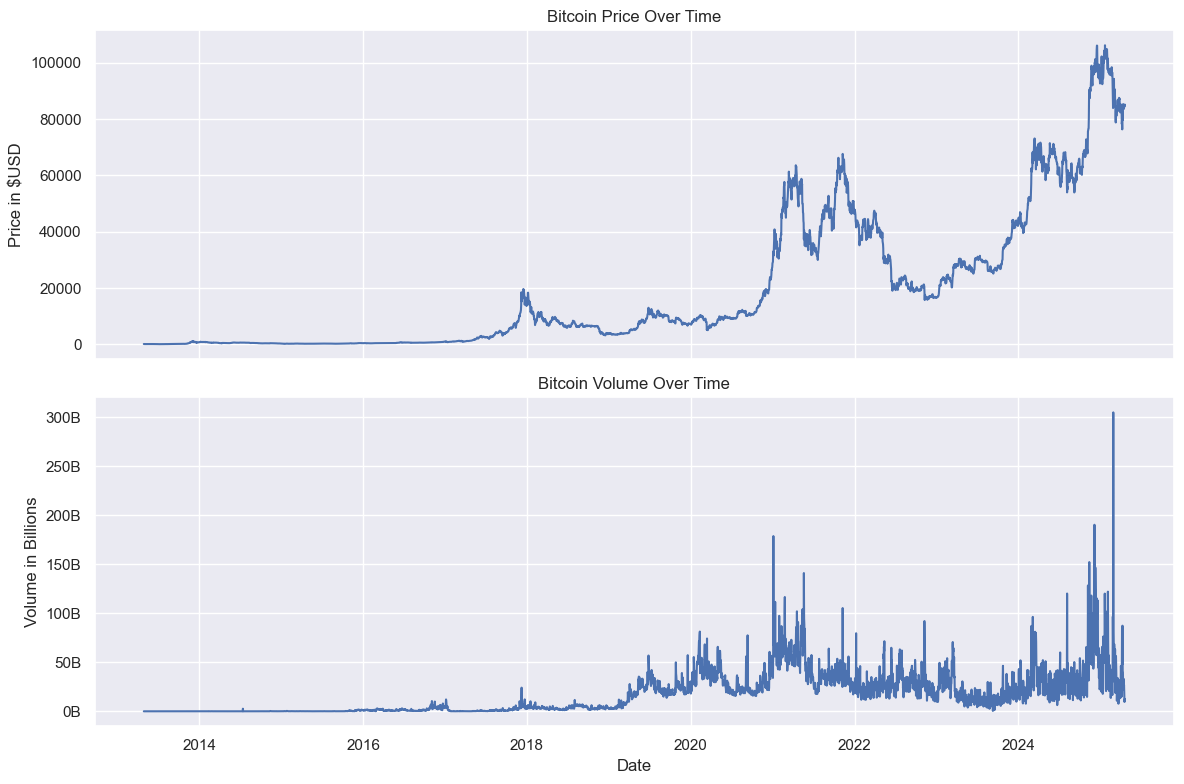
\includegraphics[width=0.8\textwidth]{Bitcoin_price_volume.png}
    \caption{Daily Bitcoin trading volume over time.}
    \label{fig:btc-volume}
\end{figure}

The figure illustrates the daily trading volume and price of Bitcoin over time.
 A notable simultaneous peak in both price and volume occurred at the end of 2024, with Bitcoin reaching an all-time high of \$109,114.88 and recording a daily trading volume exceeding \$300 billion. Additionally, the chart reveals data limitations in the earlier years, particularly between 2013 and 2014, where trading volume data is absent.
 These omissions, attributed to historical data availability issues, were addressed in Section~\ref{ch:datacollection}.

\subsubsection{Price History of Tezos}
\label{sec:xtz-pricehistory}
\begin{figure}[H]
    \centering
    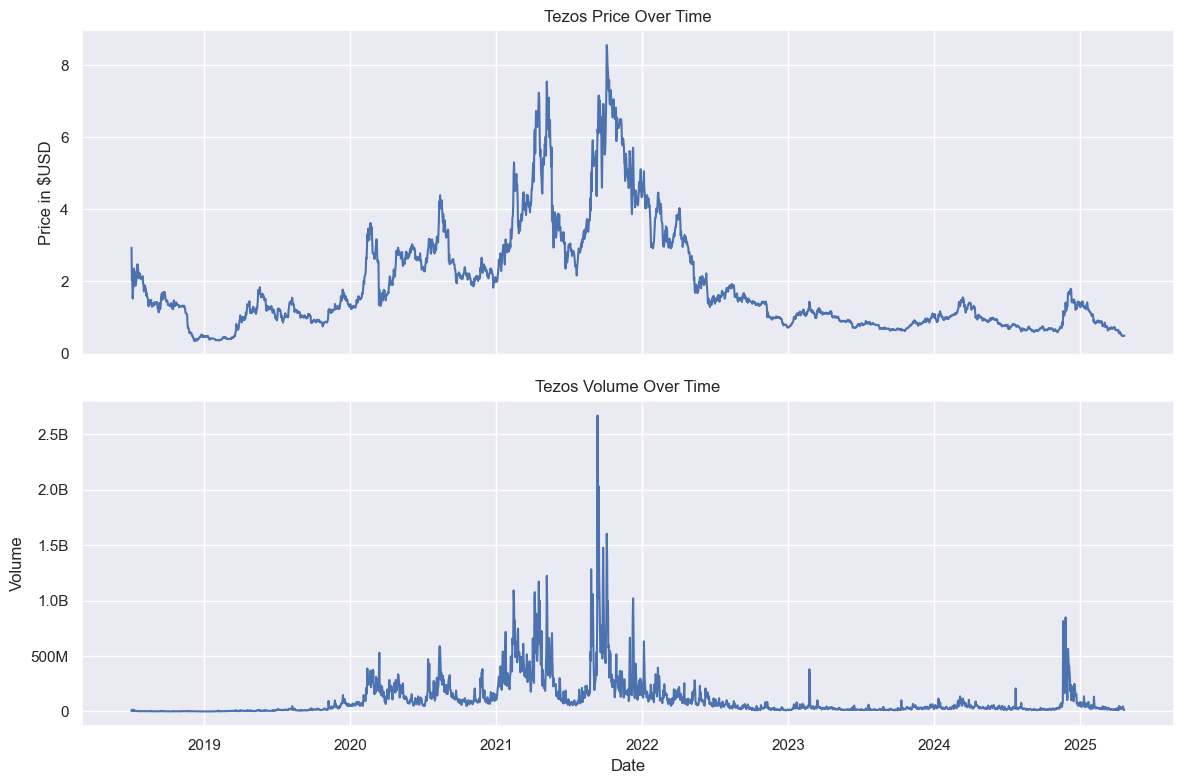
\includegraphics[width=0.8\textwidth]{Tezos_price_volume.png}
    \caption{Daily Tezos trading volume over time.}
    \label{fig:xtz-volume}
\end{figure}
The chart depicting Tezos's historical price and trading volume reveals a clear trend: both metrics generally increased until late 2021, after which they began to decline.
 Trading volume shows a particularly pronounced upward trajectory from 2018 through 2021, followed by a steady reduction to relatively low levels in recent years.
  This drop suggests a significant decrease in investor interest or market activity surrounding Tezos.
   Price movements align closely with this trend, peaking at an all-time high of \$9.12 on October 4, 2021, and subsequently declining.
    While occasional upward fluctuations have occurred—often in tandem with broader market rallies—the current price of Tezos remains considerably lower compared to its historical peak. 
    This observation underscores the diminished market enthusiasm for Tezos in the post-2021 period.

\subsubsection{Visualizing prices as a percentage of the All-Time High}
\label{sec:pricehistory-ATH}
\begin{figure}[H]
    \centering
    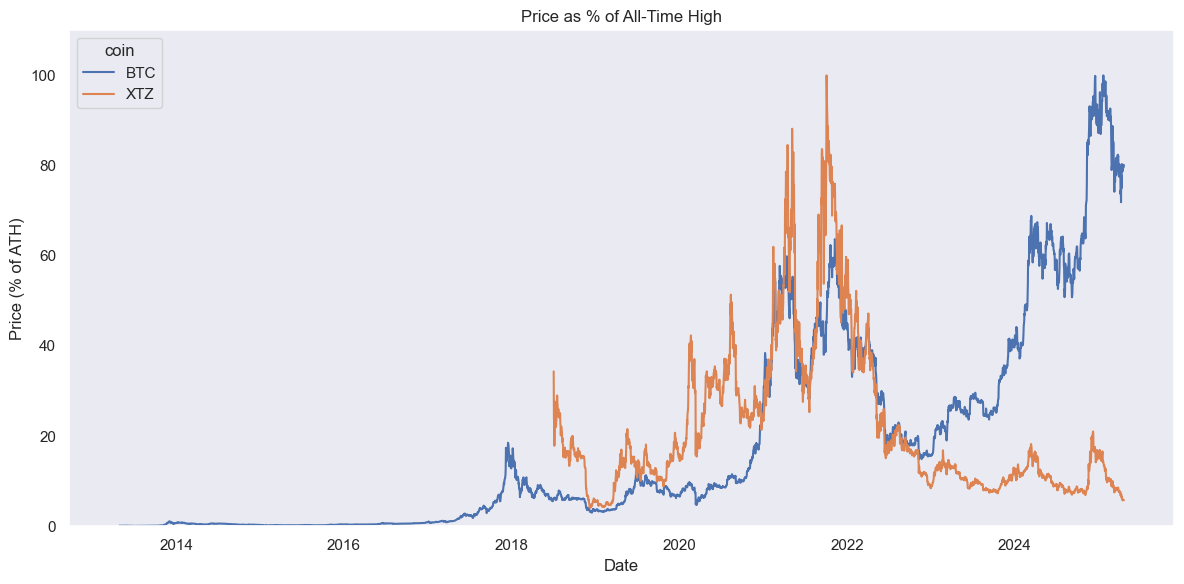
\includegraphics[width=0.8\textwidth]{athpercentage.png}
    \caption{Price of Bitcoin and Tezos as a percentage of their all-time high.}
    \label{fig:athpercentage}
\end{figure}

A common method to visualize the price history of assets is to express their prices as a percentage of their all-time high (ATH). we do this by dividing the price at each point in time by the ATH and multiplying by 100. This approach allows for a more intuitive comparison of price movements over time, regardless of the absolute price levels of the assets.
this is coded as follows:
\begin{lstlisting}[language=Python, caption={Price as a percentage of the all-time high}, label={lst:athpercentage-code}]
    dfBTC['price_pct_ath'] = dfBTC['price'] / dfBTC['price'].max() * 100
dfXTZ['price_pct_ath'] = dfXTZ['price'] / dfXTZ['price'].max() * 100
dfBTC['coin'] = 'BTC'
dfXTZ['coin'] = 'XTZ'

dfMerged = pd.concat([dfBTC,dfXTZ])

plt.figure(figsize=(12, 6))
sns.lineplot(data=dfMerged, x='date', y='price_pct_ath', hue='coin')
plt.title('Price as % of All-Time High')
plt.xlabel('Date')
plt.ylabel('Price')
plt.ylim(0, 110)
plt.tight_layout()
plt.show()
\end{lstlisting}

Figure~\ref{fig:athpercentage} presents the price trajectories of Bitcoin and Tezos expressed as a percentage of their respective all-time highs.
This normalization offers a clearer comparative perspective on the relative performance and volatility of the two assets over time. Both cryptocurrencies exhibit a broadly similar pattern, including the pronounced upward movement during the 2020–2021 bull market, followed by a period of decline.
Despite these overarching similarities, the two assets differ significantly in terms of scale and timing of price movements.
For example, there are periods in which Tezos reaches its all-time high while Bitcoin experiences only a moderate upward trend, and conversely, instances where Bitcoin achieves new record highs while Tezos displays only modest gains. These discrepancies highlight the distinct market dynamics and investor behavior influencing each asset, even within shared macroeconomic conditions.

It is also worth noting the disparity in dataset length: while Bitcoin’s historical data spans back to 2013, Tezos data begins only in mid-2018. Given that the central objective of this thesis is to predict Tezos’s price movements, the Bitcoin dataset will be truncated accordingly.

\subsubsection{Price Correlation}
\label{sec:pricecorrelation}

\begin{lstlisting}[language=Python, caption={Correlation matrix}, label={lst:correlation}]
    correlation = dfBTCfiltered['price'].corr(dfXTZfiltered['price'])
    print(correlation) #output: -0.3923556645977417
\end{lstlisting}
To examine the relationship between the daily prices of Bitcoin and Tezos, we compute the Pearson correlation coefficient.
This statistical measure quantifies the linear association between the two time series, helping to assess whether the assets tend to move together or independently. The resulting value of approximately $-0.39$ suggests a weak negative correlation, indicating that, over the examined period, the two cryptocurrencies do not consistently follow the same directional trend.

\begin{figure}[H]
    \centering
    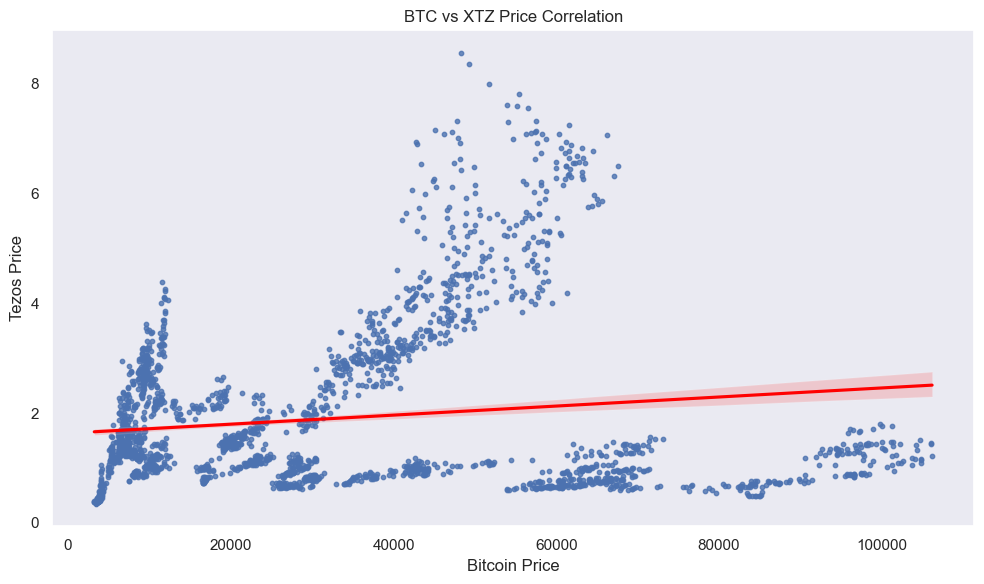
\includegraphics[width=0.85\textwidth]{scatter_price_corr.png}
    \caption{Scatter plot showing the relationship between Bitcoin and Tezos prices. A fitted regression line is included to indicate the overall trend.}
    \label{fig:price_scatter}
\end{figure}

Figure~\ref{fig:price_scatter} illustrates the relationship between the daily prices of Bitcoin and Tezos, with each point representing a single day—Bitcoin's price on the $x$-axis and Tezos's price on the $y$-axis.
 At first glance, the scatter plot appears to suggest a weak upward trend. However, the Pearson correlation coefficient of $-0.39$ indicates a moderate negative linear relationship between the two price series. 
 This apparent contradiction may be attributed to the significant difference in price scales, the clustering of data points, and potential non-linear dynamics that are not well captured by a linear trend line. 
 This emphasizes the need to supplement visual analysis with statistical measures when assessing the relationships between financial variables.
\chapter{\IfLanguageName{dutch}{Machine Learning Modellen}{Machine Learning Models}}
\label{ch:machinelearningmodels}

\section{Overview}
\label{sec:overview}

In this study, three machine learning models were selected to analyze the price dynamics of Bitcoin and Tezos. These models were chosen for their ability to capture different types of relationships in the data and their established performance in similar financial prediction tasks.

\subsection{Linear Regression}
Linear Regression serves as a baseline model. It provides a simple and interpretable way to estimate the relationship between the input features and the target variable.
 Despite its simplicity, it establishes a benchmark against which more complex models can be compared.

\subsection{Random Forest}
Random Forest was selected to capture potential non-linear relationships that cannot be modeled by linear regression.
 As an ensemble learning method based on decision trees, Random Forest is known for its robustness, resistance to overfitting, and effectiveness in handling datasets with complex interactions. Its strong performance such as in \textcite{akyildirim2021prediction} motivates its inclusion in this analysis.

\subsection{XGBoost}
XGBoost was chosen due to its consistent high performance in time series forecasting and financial data modeling tasks.
 It is a gradient boosting algorithm that constructs sequential trees, where each new tree attempts to correct the errors of the previous ones. 
 XGBoost is highly optimized for speed and accuracy, and has been successfully applied in multiple forecasting studies involving cryptocurrency prices such as in the study by \textcite{lauraalessandretti2018anticipating}.

\section{Linear Regression}
\label{sec:linearregression}
Linear Regression is a fundamental statistical method used to model the relationship between one or more independent variables and a continuous dependent variable. 
The model assumes a linear relationship of the form:

\[
y = \beta_0 + \beta_1 x_1 + \beta_2 x_2 + \cdots + \beta_n x_n + \varepsilon
\]

where \( y \) is the dependent variable, \( x_i \) are the independent variables, \( \beta_i \) are the model coefficients, and \( \varepsilon \) is the error term. 
The coefficients are typically estimated by minimizing the sum of squared residuals, following the ordinary least squares (OLS) method.

Linear Regression rests on several key assumptions: linearity between predictors and response, independence of errors, a constant variance of errors, and normally distributed residuals. Violations of these assumptions can reduce the reliability of inference and prediction, which is particularly relevant in financial time series data like cryptocurrency prices.

\subsection{Implementation}
\label{sec:linearregressionimplementation}
the Linear Regression model was implemented using the \texttt{LinearRegression} class from the \texttt{sklearn.linear\_model} module. 
First the data was split into training and testing sets, with 80\% of the data used for training and 20\% for testing like so:
\begin{lstlisting}[language=Python, caption={Splitting the data into training and testing sets}, label={lst:linearregression-split}]
  X_train, X_test, y_train, y_test = train_test_split(
    features, target, test_size=0.2, shuffle=False
)
\end{lstlisting}
Because the data is time series data, we set \texttt{shuffle=False} to maintain the temporal order of the data. 

Since Linear Regression is sensitive to feature scaling, standarization was applied to the features using the \texttt{StandardScaler} class from the \texttt{sklearn.preprocessing} module.
\begin{lstlisting}[language=Python, caption={Standardizing the features}, label={lst:linearregression-standardization}]
  scaler = StandardScaler()
  X_train_lr = scaler.fit_transform(X_train_lr)
  X_test_lr = scaler.transform(X_test_lr)
\end{lstlisting}
This ensures that the features have a mean of 0 and a standard deviation of 1, which is important for the convergence of the optimization algorithm used in Linear Regression.

\subsection{Model Training and Evaluation}
\label{sec:linearregression-training}
The model was trained using the \texttt{fit} method, which estimates the coefficients of the linear regression model based on the training data.
\begin{lstlisting}[language=Python, caption={Training the Linear Regression model}, label={lst:linearregression-training}]
  
model = LinearRegression()
model.fit(X_train_lr, y_train_lr)

y_pred_lr = model.predict(X_test_lr)

feature_names = X_train.columns

rmse_lr = np.sqrt(mean_squared_error(y_test_lr, y_pred_lr))
r2_lr = r2_score(y_test_lr, y_pred_lr)

print("RMSE:", rmse_lr)
print("R² Score:", r2_lr)

coef_df = pd.DataFrame({
    'Feature': feature_names,
    'Coefficient': model.coef_
})
coef_df['AbsCoefficient'] = coef_df['Coefficient'].abs()
coef_df = coef_df.sort_values(by='AbsCoefficient', ascending=False)
print(coef_df)

\end{lstlisting}

The model was evaluated using the root mean squared error (RMSE) and the coefficient of determination ($R^2$ score).

\begin{table}[H]
\centering
\caption{Linear Regression Performance Metrics}
\label{tab:linearregression-performance}
\begin{tabular}{lcc}
\toprule
\textbf{Metric} & \textbf{Train Set} & \textbf{Test Set} \\
\midrule
RMSE           & 0.2471             & 0.0857            \\
$R^2$ Score    & 0.9743             & 0.9085            \\
\bottomrule
\end{tabular}
\end{table}

Table \ref{tab:linearregression-performance} summarizes the performance of the linear regression model on both the training and test sets. 
The relatively low RMSE and high $R^2$ on the test set suggest that the model generalizes reasonably well, although the gap in RMSE between training and test could indicate mild overfitting or variance in the underlying data.

\subsection{Feature Importance}
\begin{table}[H]
\centering
\caption{Top 15 Linear Regression Coefficients by Absolute Value}
\label{tab:linearregression-coefficients}
\begin{tabular}{lrr}
\toprule
\textbf{Feature} & \textbf{Coefficient} & \textbf{Absolute Value} \\
\midrule
btc\_market\_cap\_3d\_ago & -6.4437 & 6.4437 \\
btc\_price\_3d\_ago       & 6.3309  & 6.3309 \\
btc\_price\_5d\_ago       & -5.3298 & 5.3298 \\
btc\_market\_cap\_5d\_ago & 5.2231  & 5.2231 \\
xtz\_price\_prev\_day     & 1.1795  & 1.1795 \\
btc\_market\_cap\_4d\_ago & 1.1629  & 1.1629 \\
btc\_price\_4d\_ago       & -1.1080 & 1.1080 \\
xtz\_market\_cap\_2d\_ago & -0.9923 & 0.9923 \\
btc\_price\_2d\_ago       & 0.9816  & 0.9816 \\
btc\_market\_cap\_2d\_ago & -0.9355 & 0.9355 \\
xtz\_price\_2d\_ago       & 0.8347  & 0.8347 \\
xtz\_market\_cap\_3d\_ago & 0.4663  & 0.4663 \\
xtz\_price\_3d\_ago       & -0.3381 & 0.3381 \\
xtz\_price\_4d\_ago       & -0.1679 & 0.1679 \\
xtz\_market\_cap\_prev\_day & 0.1474 & 0.1474 \\
\bottomrule
\end{tabular}
\end{table}

Given the simplicity of Linear Regression and the relatively small number of input features, the risk of overfitting is minimal. 
This is supported by the model’s stable performance on the test set, indicating that it generalizes well to unseen data. 
The design of the feature set also played a crucial role in guaranteeing a fair evaluation: all variables were lagged appropriately to avoid any form of data leakage or lookahead bias (see Code snippet~\ref{lst:linearregression-lagged}).
\begin{lstlisting}[language=Python, caption={Lagged features}, label={lst:linearregression-lagged}]
  # Add target (Tezos price tomorrow)
  df['xtz_target'] = df['xtz_price'].shift(-1)
\end{lstlisting}

 Only information that would have been available at the time of prediction was used during training. 
 The computed coefficients (see Table~\ref{tab:linearregression-coefficients}) provide insight into how the model weights each input variable, offering a clear picture of the linear relationships it has learned. This coefficient-based structure makes Linear Regression particularly transparent and easy to evaluate, even if its simplicity limits its ability to model more complex interactions within the data.

\subsection{Result}
\begin{figure}[H]
    \centering
    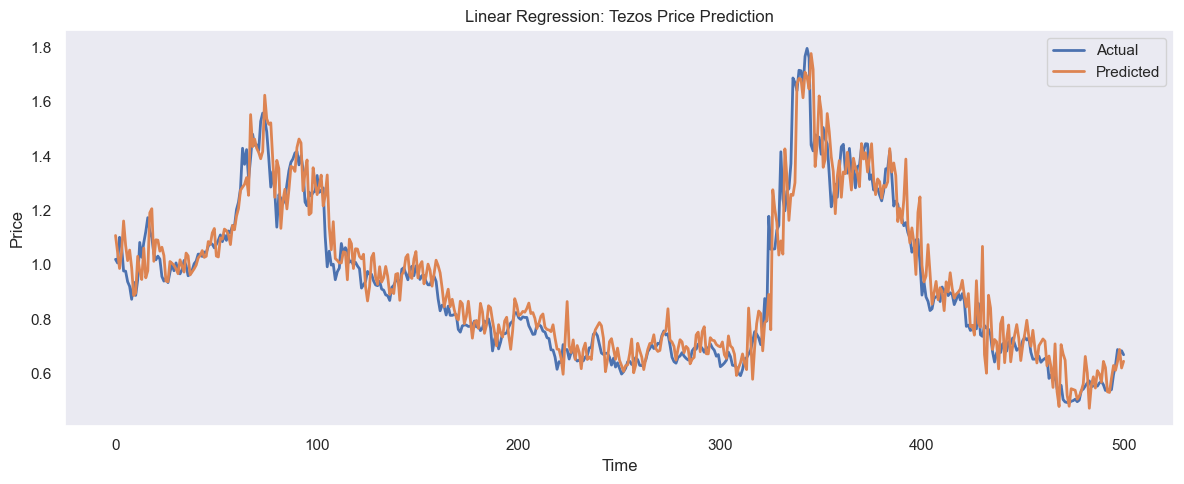
\includegraphics[width=0.8\textwidth]{LinearRegressionTezos.png}
    \caption{Linear Regression: Predicted vs Actual Tezos Price}
    \label{fig:linearregression-tezos}
\end{figure}

\subsection{Model Interpretation}
\label{sec:linearregression-interpretation}

Despite its simplicity, the Linear Regression model delivered strong predictive performance, achieving a test RMSE of approximately 0.0857 and an $R^2$ score of around 0.9085.
The model assumes a fixed linear relationship between the input features and the target variable, which is a strong constraint in the context of financial time series data, known for their volatility and nonlinear interactions. Nonetheless, the linear model managed to capture a substantial portion of the variation in Tezos price movements. 
This is particularly notable given that it neither incorporates lagged nonlinear interactions nor benefits from ensemble methods or decision trees.
As shown in Table~\ref{tab:linearregression-coefficients}, the most influential features were lagged values of Bitcoin and Tezos price and market capitalization, with \texttt{btc\_market\_cap\_3d\_ago}, \texttt{btc\_price\_3d\_ago}, and \texttt{btc\_price\_5d\_ago} having the highest absolute coefficients. 
This suggests that the model's predictive capacity stems primarily from lagged features in both assets. \texttt{xtz\_price\_prev\_day} also had a substantial influence on the model’s predictions, which is consistent with expectations in financial models where recent price levels often dominate due to short-term momentum and persistence.
Bitcoin-related variables showed some influence, but their effects appear more indirect and less consistent. These findings align with the expectation that in autoregressive contexts, past prices—especially of closely linked assets—can act as useful predictors. However, the linear structure limits the model’s ability to capture more complex or conditional relationships.
The model captures the overall trend reasonably well but struggles during rapid price shifts. This is likely because a linear model can’t adapt to sudden changes or nonlinear patterns in the data, which require more flexible approaches to model effectively.
Overall, the Linear Regression model sets a strong baseline and offers a useful lens through which the influence of lagged variables can be assessed. Further comparison with more complex models will help determine whether the added complexity meaningfully enhances predictive accuracy or merely introduces risk of overfitting.

\section{Random Forest Regression}
The random forest regression model is an ensemble learning method that constructs multiple decision trees during training and outputs the average prediction of the individual trees.
It was chosen for its ability to capture complex, non-linear relationships in the data and its robustness against overfitting aswell as its great performance in the study by \textcite{akyildirim2021prediction} .

\subsection{Implementation}
The Random Forest Regressor was implemented using the \texttt{RandomForestRegressor} class from the \texttt{sklearn.ensemble} module. 
This estimator builds an ensemble of decision trees and aggregates their predictions to improve generalization and reduce overfitting.
No feature scaling was applied, as decision trees are not sensitive to the scale of the input features. 
The data was again split into training and testing sets, using 80\% for training and 20\% for testing, with shuffling disabled to preserve the chronological order of the time series (see Code snippet~\ref{lst:linearregression-split}).

\subsection{Model Training and Evaluation}
To find a suitable set of hyperparameters, a randomized search was performed using \texttt{RandomizedSearchCV} in combination with \texttt{TimeSeriesSplit}. A randomized search is a more efficient alternative to grid search, as it samples a fixed number of hyperparameter combinations from a specified distribution, rather than exhaustively searching through all possible combinations.
It does this by randomly selecting a subset of hyperparameters from a predefined grid, which allows for a more efficient exploration of the hyperparameter space.

\texttt{TimeSeriesSplit} was used for cross-validation because it respects the temporal order of the data, preventing information leakage from future data points into past training folds—a crucial consideration when working with time series data. 
This ensures that model evaluation more realistically reflects its performance on unseen future data.

\begin{lstlisting}[language=Python, caption={Training the Random Forest Model}, label={lst:randomforest-training}]
  param_dist = {
    'n_estimators': randint(100, 501),
    'max_depth': randint(3, 15),
    'min_samples_split': randint(2, 10),
    'min_samples_leaf': randint(1, 5),
    'max_features': ['auto', 'sqrt', 'log2']
}

# TimeSeriesSplit to respect temporal ordering
tscv = TimeSeriesSplit(n_splits=5)

rf = RandomForestRegressor(random_state=42)

search = RandomizedSearchCV(
    estimator=rf,
    param_distributions=param_dist,
    n_iter=50,
    scoring='neg_mean_squared_error',
    cv=tscv,
    random_state=42,
    verbose=1,
    n_jobs=-1
)

# Fit on training data only
search.fit(X_train_rf, y_train_rf)

# Evaluate on held-out test data
best_rf = search.best_estimator_
y_pred_rf = best_rf.predict(X_test_rf)

rmse_rf = np.sqrt(mean_squared_error(y_test_rf, y_pred_rf))
r2_rf = r2_score(y_test_rf, y_pred_rf)

print("Best Parameters:", search.best_params_)
print(f"Tuned RF RMSE: {rmse_rf:.4f}")
print(f"Tuned RF R² Score: {r2_rf:.4f}")
\end{lstlisting}

In the code snippet above (see Code Snippet~\ref{lst:randomforest-training}), we perform 50 iterations of randomized search over the hyperparameter space defined in the \texttt{param\_dist} object. 
Multiple values for \texttt{n\_iter} have been tested, but 50 iterations were found to be sufficient to identify a strong set of hyperparameters without excessive computational cost.
To keep the random search reproducible, a fixed random seed was set using \texttt{random\_state=42}.
The best hyperparameters were selected based on the lowest negative mean squared error (NMSE) across the cross-validation folds.

The final model was trained using the following parameters:
\begin{table}[H]
\centering
\caption{RandomForestRegressor Parameters}
\label{tab:randomforest-parameters}
\begin{tabular}{lr}
\toprule
\textbf{Parameter} & \textbf{Value} \\
\midrule
\texttt{n\_estimators} & 437 \\
\texttt{max\_depth} & 10 \\
\texttt{max\_features} & \texttt{auto} \\
\texttt{min\_samples\_split} & 6 \\
\texttt{min\_samples\_leaf} & 4 \\
\bottomrule
\end{tabular}
\end{table}

\begin{table}[H]
\centering
\caption{RandomForestRegressor Performance Metrics}
\label{tab:randomforest-performance}
\begin{tabular}{lcc}
\toprule
\textbf{Metric} & \textbf{Train Set} & \textbf{Test Set} \\
\midrule
RMSE           & 0.1443             & 0.0810            \\
$R^2$ Score    & 0.9912             & 0.9182            \\
\bottomrule
\end{tabular}
\end{table}

The Random Forest model shows strong performance on both training and test sets, with an $R^2$ score of 0.9912 on training data and 0.9182 on the test set. 
While the drop does suggest mild overfitting, the gap is not dramatic—indicating that the model generalizes reasonably well. 
The low test RMSE of 0.0810 supports this, reflecting the model’s ability to track Tezos price movements with high accuracy. 
However, the strong training fit also points to a tendency to memorize patterns, particularly when fluctuations are small. 
These results likely stem from the model’s strength in capturing stable price behavior, though its ability to adapt during more volatile periods remains limited.


\subsection{Feature Importance}
\begin{table}[H]
\centering
\caption{Top 15 Random Forest Feature Importances}
\label{tab:randomforest-feature-importance}
\begin{tabular}{lr}
\toprule
\textbf{Feature} & \textbf{Importance} \\
\midrule
\texttt{xtz\_price\_prev\_day}   & 0.9633 \\
\texttt{xtz\_price\_2d\_ago}     & 0.0124 \\
\texttt{xtz\_market\_cap\_prev\_day} & 0.0066 \\
\texttt{xtz\_price\_3d\_ago}     & 0.0017 \\
\texttt{btc\_volume\_2d\_ago}    & 0.0011 \\
\texttt{btc\_volume\_5d\_ago}    & 0.0011 \\
\texttt{btc\_volume\_prev\_day}  & 0.0009 \\
\texttt{xtz\_price\_5d\_ago}     & 0.0008 \\
\texttt{xtz\_price\_4d\_ago}     & 0.0008 \\
\texttt{btc\_price\_3d\_ago}     & 0.0008 \\
\texttt{xtz\_volume\_prev\_day}  & 0.0007 \\
\texttt{xtz\_volume\_5d\_ago}    & 0.0007 \\
\texttt{xtz\_volume\_4d\_ago}    & 0.0007 \\
\texttt{btc\_volume\_3d\_ago}    & 0.0007 \\
\texttt{xtz\_market\_cap\_3d\_ago} & 0.0006 \\
\bottomrule
\end{tabular}
\end{table}

In terms of Feature Importance, the Random Forest model showed a strong preference for \texttt{xtz\_price\_prev\_day}, which accounted for 96.33\% of the total importance (see Table~\ref{tab:randomforest-feature-importance}).


\subsection{Result}
\begin{figure}[H]
    \centering
    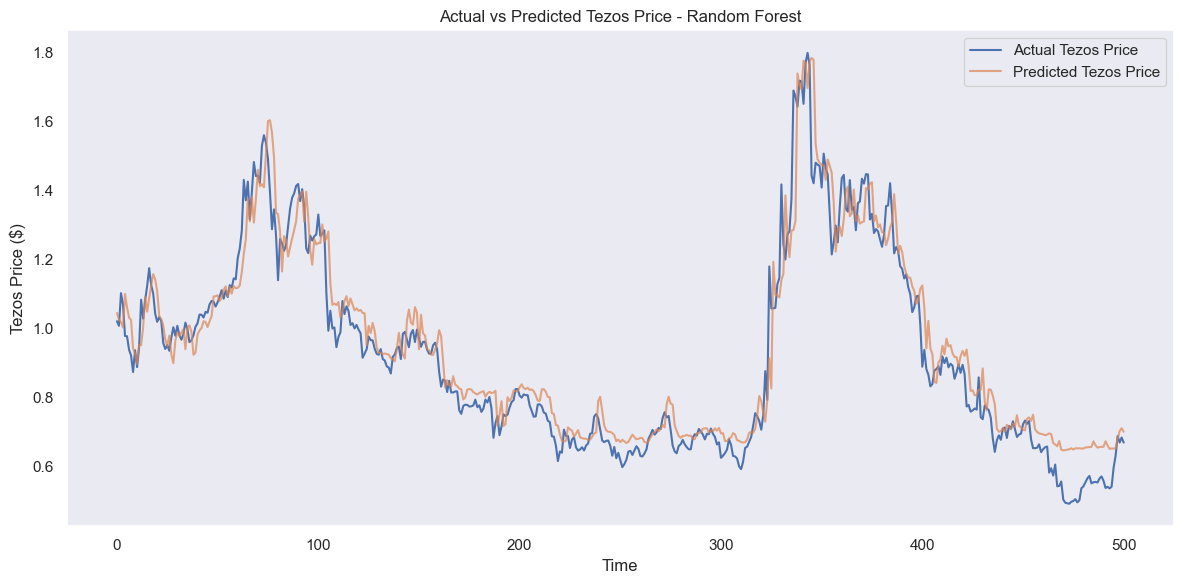
\includegraphics[width=0.8\textwidth]{RandomForestTezos.png}
    \caption{Random Forest Regression: Predicted vs Actual Tezos Price}
    \label{fig:randomforest-tezos}
\end{figure}

\subsection{Model Interpretation}

The Random Forest model demonstrated strong predictive accuracy, achieving a root mean squared error (RMSE) of 0.0810 and an $R^2$ score of 0.9182 on the test set. 
These results indicate that the model successfully captures the underlying patterns in the data and improves upon the performance of the linear regression approach.
A closer examination of feature importance values in Table~\ref{tab:randomforest-feature-importance} shows that this performance is driven almost entirely by a single predictor: \texttt{xtz\_price\_prev\_day}, which accounts for approximately 96.33\% of the total importance. 
This result is not surprising. In financial time series, the most recent price is typically a strong predictor of future values due to inherent autocorrelation and momentum effects.
What stands out, however, is the magnitude of this dominance.
The model assigns negligible importance to all other features—such as \texttt{xtz\_volume\_prev\_day}, \texttt{btc\_volume\_prev\_day}, and \texttt{xtz\_market\_cap\_prev\_day}—each contributing essentially 0\%. 
This suggests that, given the current set of predictors and the model architecture, Bitcoin-related variables offer little to no additional predictive value when forecasting Tezos prices. What this also indicates is that the model is primarily capturing short-term momentum in Tezos prices, rather than any complex interactions or relationships with Bitcoin price or other features.
Because of this overwhelming reliance on a single feature, the model's interpretability is limited. 
Compared to the Linear Regression model, the Random Forest model—despite its greater complexity—does not appear to uncover richer or more nuanced relationships between features. 
Notably, features such as \texttt{btc\_market\_cap\_3d\_ago}, \texttt{btc\_price\_3d\_ago}, \texttt{btc\_price\_5d\_ago}, and \texttt{btc\_market\_cap\_5d\_ago} were assigned very large coefficients in the linear model (see Table~\ref{tab:linearregression-coefficients}), suggesting a consistent linear influence. 
However, these same features receive minimal importance in the Random Forest model. This discrepancy likely stems from the Random Forest model’s tendency to prioritize nonlinear splits and interactions, which may cause it to overlook subtle but consistent linear relationships that are more directly captured by a linear model.

\section{XGBoost}
\label{sec:xgboost}
XGBoost is a machine learning algorithm that belongs to the ensemble learning category, specifically the gradient boosting framework. 
It utilizes decision trees as base learners and employs regularization techniques to enhance model generalization.
It’s the go-to algorithm for a wide range of tasks, including regression, classification, and ranking. (\cite{tyagi2025xgboost})

\subsection{Implementation}
\label{sec:xgboost-implementation}
The XGBoost model was implemented using the \texttt{xgboost} library. This library is widely used for its scalability, efficiency, and state-of-the-art performance on structured data. 
XGBoost builds on the standard gradient boosting framework by adding features like L1 and L2 regularization, learning rate shrinkage, and efficient tree pruning. 
While its built-in handling of missing values isn’t relevant here, these enhancements help prevent overfitting and improve performance, especially when working with many potentially weakly informative features.
The data was again split into training and testing sets, using 80\% for training and 20\% for testing, with shuffling disabled to preserve the chronological order of the time series (see Code snippet~\ref{lst:linearregression-split}).

\subsection{Model Training and Evaluation}
\label{sec:xgboost-training}
To identify a suitable set of hyperparameters, we once again use \texttt{RandomizedSearchCV} in combination with \texttt{TimeSeriesSplit}. 
This approach avoids data leakage and provides a more realistic estimate of model performance in time series contexts.
The hyperparameters \texttt{n\_estimators}, \texttt{learning\_rate}, \texttt{max\_depth}, \texttt{colsample\_bytree}, \texttt{subsample}, \texttt{gamma}, and \texttt{min\_child\_weight} were systematically tuned to strike a balance between bias and variance.

\begin{lstlisting}[language=Python, caption={Training the XGBoost Model}, label={lst:xgboost-training}]
param_distributions = {
    'min_child_weight': randint(1, 11),
    'gamma': uniform(0, 1),
    'n_estimators': randint(100, 501),
    'max_depth': randint(3, 7),
    'learning_rate': uniform(0.01, 0.09),
    'subsample': uniform(0.6, 0.4),
    'colsample_bytree': uniform(0.8, 0.2),
    'reg_alpha': uniform(0, 1),
    'reg_lambda': uniform(0.5, 1.5)
}

tscv = TimeSeriesSplit(n_splits=5)

# XGBoost regressor
xgb_model = xgb.XGBRegressor(objective='reg:squarederror', random_state=42)

# Randomized search with time series CV
random_search = RandomizedSearchCV(
    estimator=xgb_model,
    param_distributions=param_distributions,
    n_iter=500,
    scoring='neg_mean_squared_error',
    cv=tscv,
    verbose=1,
    n_jobs=-1,
    random_state=42
)

random_search.fit(X_train_xgb, y_train_xgb)

xgb_model = random_search.best_estimator_
y_pred_xgb = xgb_model.predict(X_test_xgb)

rmse_xgb = np.sqrt(mean_squared_error(y_test_xgb, y_pred_xgb))  # RMSE
r2_xgb = r2_score(y_test_xgb, y_pred_xgb)

print("Best parameters:", random_search.best_params_)
print("Best CV score (negative MSE):", random_search.best_score_)
print(f"Tuned XGBoost RMSE: {rmse_xgb:.4f}")
print(f"Tuned XGBoost R² Score: {r2_xgb:.4f}")
\end{lstlisting}

The final model was trained using the following parameters:
\begin{table}[H]
\centering
\caption{Tuned XGBoost Parameters (rounded to 4 decimal places)}
\label{tab:xgboost-parameters}
\begin{tabular}{lr}
\toprule
\textbf{Parameter} & \textbf{Value} \\
\midrule
\texttt{colsample\_bytree} & 0.8116 \\
\texttt{gamma} & 0.1115 \\
\texttt{learning\_rate} & 0.0564 \\
\texttt{max\_depth} & 6 \\
\texttt{min\_child\_weight} & 5 \\
\texttt{n\_estimators} & 173 \\
\texttt{subsample} & 0.7349 \\
\texttt{reg\_alpha} & 0.0146 \\
\texttt{reg\_lambda} & 1.0686 \\
\bottomrule
\end{tabular}
\end{table}

\begin{table}[H]
\centering
\caption{XGBoost Performance Metrics}
\label{tab:xgboost-performance}
\begin{tabular}{lcc}
\toprule
\textbf{Metric} & \textbf{Train Set} & \textbf{Test Set} \\
\midrule
RMSE           & 0.1117             & 0.1127            \\
$R^2$ Score    & 0.9948             & 0.8415            \\
\bottomrule
\end{tabular}
\end{table}

The XGBoost model achieved an excellent fit on the training set, with an $R^2$ score of 0.9948 and an RMSE of 0.1117.
However, this strong in-sample performance does not extend to the test set, where the $R^2$ drops to 0.8415 and the RMSE increases to 0.1127—worse than that of the Random Forest model. 
This substantial gap between training and test results is a clear indication of overfitting: the model learns the training data exceptionally well but struggles to generalize to new data.
One possible explanation for this overfitting is the amount of feature noise present in the dataset, Too many features can have a negative impact on model performance, especially when many features are weakly informative or irrelevant.

Notably, this pattern persisted even when the model was retrained using fewer estimators and simpler configurations. 
Reducing model complexity did little to improve generalization, suggesting that the performance bottleneck may not be due to overparameterization alone. 
Instead, it could reflect the limitations of the available features or the underlying signal-to-noise ratio in the data.

\subsection{Feature Importance}
\begin{table}[H]
\centering
\caption{Top 15 XGBoost Feature Importances}
\label{tab:xgboost-feature-importance}
\begin{tabular}{lr}
\toprule
\textbf{Feature} & \textbf{Importance} \\
\midrule
\texttt{xtz\_price\_2d\_ago}       & 0.3894 \\
\texttt{xtz\_price\_prev\_day}     & 0.3878 \\
\texttt{xtz\_market\_cap\_prev\_day} & 0.0662 \\
\texttt{xtz\_price\_3d\_ago}       & 0.0465 \\
\texttt{xtz\_market\_cap\_3d\_ago} & 0.0101 \\
\texttt{xtz\_price\_5d\_ago}       & 0.0096 \\
\texttt{xtz\_price\_4d\_ago}       & 0.0089 \\
\texttt{xtz\_market\_cap\_2d\_ago} & 0.0069 \\
\texttt{btc\_market\_cap\_prev\_day} & 0.0054 \\
\texttt{btc\_volume\_5d\_ago}      & 0.0050 \\
\texttt{btc\_price\_4d\_ago}       & 0.0045 \\
\texttt{btc\_price\_prev\_day}     & 0.0044 \\
\texttt{btc\_price\_5d\_ago}       & 0.0040 \\
\texttt{btc\_volume\_prev\_day}    & 0.0040 \\
\texttt{btc\_market\_cap\_2d\_ago} & 0.0039 \\
\bottomrule
\end{tabular}
\end{table}

The XGBoost model’s feature importance scores (see Table~\ref{tab:xgboost-feature-importance}) mirror the pattern observed in the Random Forest model, though here two features dominate instead of one. \texttt{xtz\_price\_2d\_ago} and \texttt{xtz\_price\_prev\_day} together account for approximately 77.2\% of the total importance, highlighting the model’s strong dependence on recent Tezos price movements. This closely aligns with the Random Forest results, where predictive power is likewise concentrated in short-term price history.

\subsection{Result}
\begin{figure}[H]
    \centering
    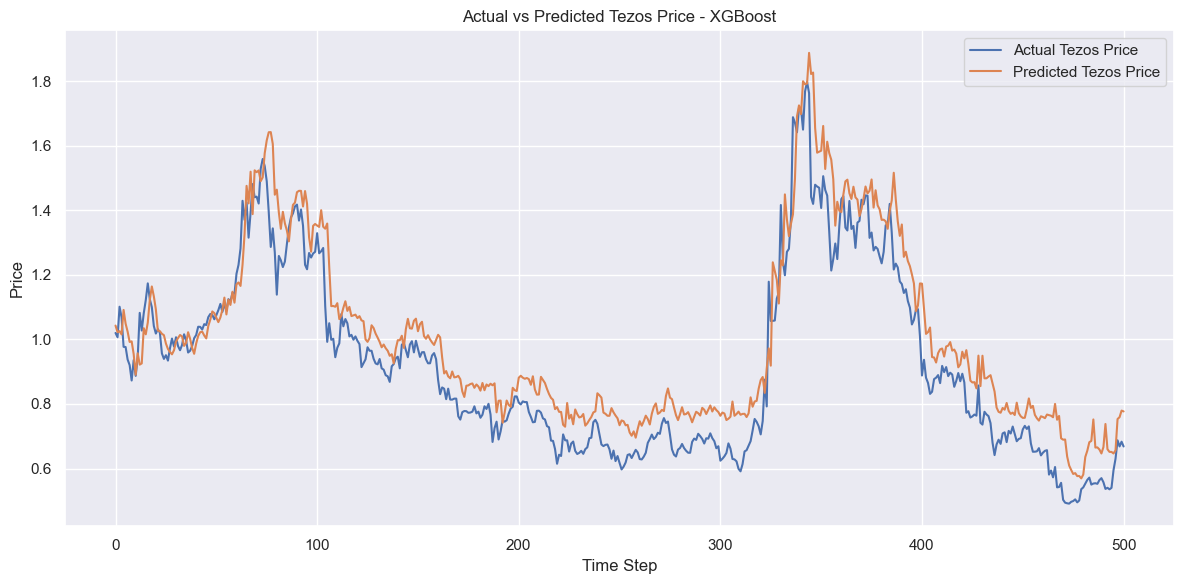
\includegraphics[width=0.8\textwidth]{xgboostTezos.png}
    \caption{XGBoost: Predicted vs Actual Tezos Price}
    \label{fig:xgboost-tezos}
\end{figure}

\subsection{Model Interpretation}
\label{sec:xgboost-interpretation}

The XGBoost model underperformed relative to both the Random Forest and Linear Regression models, achieving a test RMSE of 0.1127 and an $R^2$ score of 0.8415. This represents a notable drop in predictive accuracy compared to the Random Forest model and suggests a degree of overfitting, despite extensive hyperparameter tuning efforts. Attempts to regularize the model by reducing complexity did little to improve generalization, indicating that performance limitations are likely rooted in the data itself, rather than the model configuration.

As shown in Table~\ref{tab:xgboost-feature-importance}, the model’s predictions are overwhelmingly dominated by two features: \texttt{xtz\_price\_2d\_ago} and \texttt{xtz\_price\_prev\_day}, which together account for approximately 77\% of the total importance. This mirrors the pattern seen in the Random Forest model, where a single recent price dominated. The remaining features, particularly all Bitcoin-related variables, contribute virtually nothing—many with importance values indistinguishable from noise.

This strongly suggests that, within the current dataset, the model has not learned any meaningful cross-asset relationships. In contrast, the Linear Regression model assigned large coefficients to certain Bitcoin-related features (e.g., \texttt{btc\_market\_cap\_3d\_ago}, \texttt{btc\_price\_3d\_ago}), implying that consistent linear effects may exist—though their true explanatory value remains questionable given the poor performance of more flexible models.

Overall, XGBoost added no value in terms of accuracy or interpretability. Its capacity for modeling nonlinear interactions was not meaningfully utilized in this context, as it simply reinforced the already evident conclusion: recent Tezos prices are the only substantial drivers of short-term predictions, and most other variables—including those related to Bitcoin—are effectively redundant in this setting.

\section{Comparison of Models}
\label{sec:comparison}

\begin{figure}[H]
    \centering
    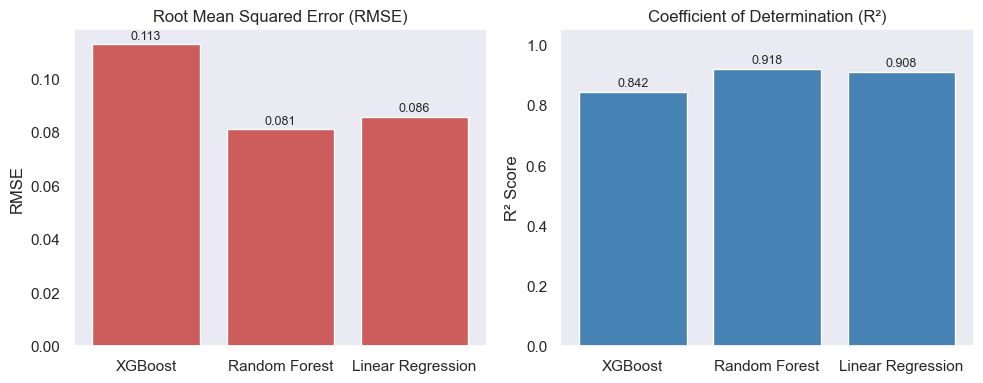
\includegraphics[width=0.8\textwidth]{modelcomparison.png}
    \caption{Comparison of Model Performance}
    \label{fig:model-comparison}
\end{figure}

In summary, each of the three models explored presents a different balance between predictive accuracy and interpretability. 
XGBoost delivered the best performance on the training data ($R^2$ of 0.9948, RMSE of 0.1117), but its test performance dropped significantly ($R^2$ of 0.8415, RMSE of 0.1127), revealing substantial overfitting and poor generalization. Random Forest performed more reliably on unseen data, achieving the lowest test RMSE (0.0810) and a strong $R^2$ of 0.9182, suggesting better generalization. However, both tree-based models focused almost exclusively on lagged Tezos price values, contributing little interpretative value regarding cross-asset relationships. 
Bitcoin-related features were effectively treated as noise, receiving near-zero importance in both cases.
In contrast, Linear Regression, while slightly less accurate (test $R^2$ of 0.9085, RMSE of 0.0857), offered substantial value from an analytical standpoint. 
It surfaced several Bitcoin-related predictors—such as \texttt{btc\_pric\_3d\_ago} and \texttt{btc\_market\_cap\_5d\_ago}—with consistently strong coefficients, indicating potential linear relationships between the two markets. 
Despite its simplicity, the model captured both autocorrelation within Tezos prices and cross-market signals, providing a more interpretable and theoretically informative view of the data. 
As such, Linear Regression not only complements the thesis aim of examining Bitcoin–Tezos dynamics, but also outperforms more complex models in offering meaningful insights—making it arguably the most valuable model for this study.
% Voeg hier je eigen hoofdstukken toe die de ``corpus'' van je bachelorproef
% vormen. De structuur en titels hangen af van je eigen onderzoek. Je kan bv.
% elke fase in je onderzoek in een apart hoofdstuk bespreken.

%\input{...}
%\input{...}
%...

%%=============================================================================
%% Conclusie
%%=============================================================================

\chapter{Conclusion}%
\label{ch:conclusion}

This study applied three machine learning models—Linear Regression, Random Forest, and XGBoost—to explore whether Bitcoin market variables can help predict short-term Tezos price movements. 
In both the Random Forest and XGBoost model, the results pointed to the same conclusion: Bitcoin-related features exhibited virtually no predictive power in this context (See Table~\ref{tab:randomforest-feature-importance} and Table~\ref{tab:xgboost-feature-importance}).
Instead, the most significant predictor across these two models was the previous Tezos price itself, which is consistent with the autoregressive behavior commonly observed in financial time series. 
Because of this over reliance on the previous Tezos price, the models mostly excelled in short-term predictions, with the Random Forest model achieving an $R^2$ score of 0.9912 on training data and 0.9182 on the test set. 
But both models struggled to generalize longer periods of time or sudden market shifts. (See Figure~\ref{fig:randomforest-tezos} and Figure~\ref{fig:xgboost-tezos}) On these figures, we can see that when the Tezos price experiences a significant drop or increase, the models fail to predict the price accurately, resulting in large prediction errors.

However, the Linear Regression model gave a different perspective, showing that a 3-day lagged Bitcoin price and market capitalization had a significant influence on Tezos price movements, with an $R^2$ score of 0.9743 on training data and 0.9085 on the test set. 
While its overall predictive accuracy was slightly lower than that of the Random Forest model, the interpretability of the linear model proved especially valuable. 
The prominence of the 3-day lagged Bitcoin features, specifically \texttt{btc\_price\_3d\_ago} and \texttt{btc\_market\_cap\_3d\_ago}, suggests that there may be a delayed linear relationship between Bitcoin and Tezos that nonlinear models failed to detect or prioritize or detect (potentially because of noise).
This kind of temporal lag is meaningful in financial modeling because it implies a potential lead-lag relationship: Bitcoin price movements could be influencing Tezos, but with a delay of several days. In real-world trading or risk management settings, identifying such delayed dependencies is extremely useful, as it allows for the anticipation of future price shifts in Tezos based on known information from the Bitcoin market. 
Unlike the tree-based models that aggressively favor the most recent data and nonlinear splits, the Linear Regression model captures more subtle, time-distributed effects that might otherwise be treated as noise. 
As such, even if its predictions are less accurate in absolute terms, its explanatory power offers deeper insight into the potential correlations between the two assets—insight that could guide both further research and decentralized exchanges such as CrunchySwap.
Because of this, the Linear Regression model serves as the most informative tool for understanding the potential relationship between Bitcoin and Tezos in this study. 
While it does not deliver the highest predictive performance, its transparent structure and interpretable coefficients allow for a clearer evaluation of individual feature contributions. 
The model's ability to highlight the predictive role of 3-day lagged Bitcoin variables, which went undetected in the more complex models, demonstrates that simpler, linear approaches can surface important but easily overlooked temporal relationships. 

Several limitations of this study should be acknowledged, particularly regarding the dataset and feature construction. 
The models were trained on a relatively limited set of features, primarily derived from historical price and volume data of Tezos and Bitcoin. While there was over 30 features engineered, including lagged values and returns, the feature set remained focused on direct price and volume metrics. 
While sufficient for testing basic autoregressive and cross-asset predictive relationships, this constrained feature space may have hindered the ability of more complex models—such as XGBoost—to demonstrate their full potential and likely explains its poor performance and inability to generalize. 
A more feature-rich dataset, incorporating additional market indicators, on-chain metrics, or engineered features such as rolling averages or volatility measures, might yield improved performance and potentially uncover more nuanced patterns.
Furthermore, the models did not account for external factors that often influence cryptocurrency price dynamics. These include market sentiment, news events, macroeconomic indicators (e.g., interest rates, inflation data), social media activity, regulatory announcements, and broader investor behavior. Incorporating such variables, particularly through sentiment analysis or natural language processing applied to Twitter, Reddit, or news headlines, could provide a more holistic view and improve predictive accuracy. 
The absence of these elements likely contributed to the inability of the non-linear models to capture more complex or indirect relationships between Bitcoin and Tezos prices.

In conclusion, although Random Forest and XGBoost delivered stronger raw predictive performance by heavily relying on recent Tezos prices, they contributed little to understanding the underlying dynamics between Bitcoin and Tezos. 
In contrast, the Linear Regression model, despite being simpler and slightly less accurate, offered more meaningful insight. Its identification of a delayed relationship between Bitcoin market variables and Tezos prices suggests the presence of a subtle, time-lagged influence that non-linear models may have ignored or dismissed as noise. 
This finding underscores the value of interpretability and temporal nuance in financial modeling. Ultimately, the study highlights that predictive accuracy alone is not sufficient: model transparency and the ability to detect economically plausible relationships are just as crucial, especially when the goal is to uncover mechanisms rather than simply forecast numbers.
Future research could expand on this work by incorporating additional data sources such as market sentiment indicators, on-chain analytics, or macroeconomic variables. 
Testing different model architectures, including recurrent neural networks—such as in studies by \textcite{mishal2022prediction} and \textcite{mallqui2019predicting},  or transformer-based approaches, could also offer deeper insight into temporal dependencies and cross-asset relationships.

\subsection{Discussion}

The poor performance of the Random Forest and XGBoost models was unexpected given their reputation for capturing complex, nonlinear dependencies—particularly in financial time series. 
These models defaulted to heavily relying on recent Tezos prices, failing to identify any meaningful influence from Bitcoin variables.
Ironically, the simplest model—Linear Regression—was the one that surfaced the most relevant insight. 
Initially included as a baseline, it revealed a statistically significant 3-day lagged relationship between Bitcoin and Tezos. This suggests that linear dependencies, when temporally distributed, may be more visible to interpretable models that don’t aggressively prioritize immediate predictors.
The results imply that predictive complexity does not guarantee explanatory value. When the goal includes uncovering potential inter-asset relationships, especially subtle ones, simpler models may not just suffice—they may outperform in terms of insight. This shift in utility from predictive to explanatory makes the case for not underestimating baseline models in exploratory financial research.


%---------- Bijlagen -----------------------------------------------------------

\appendix

\chapter{Onderzoeksvoorstel}

Het onderwerp van deze bachelorproef is gebaseerd op een onderzoeksvoorstel dat vooraf werd beoordeeld door de promotor. Dat voorstel is opgenomen in deze bijlage.

%% TODO: 
%\section*{Samenvatting}

% Kopieer en plak hier de samenvatting (abstract) van je onderzoeksvoorstel.

% Verwijzing naar het bestand met de inhoud van het onderzoeksvoorstel
%---------- Inleiding ---------------------------------------------------------

\section{Introduction}% \label{sec:Introduction}

The cryptocurrency market has undergone significant shifts recently, with Bitcoin reaching record highs and driving a surge in market cap. However, despite Bitcoin's dominance, altcoins like Tezos have not experienced the same level of growth, raising questions among traders, developers, 
and analysts about the factors that drive such disparities. This provides a valuable opportunity to explore the relationship between Bitcoin's price movements and the price dynamics of smaller blockchain ecosystems like Tezos. Understanding these relationships is especially important for decentralized exchanges, such as CrunchySwap, which operates on the Tezos blockchain and faces operational challenges tied to Tezos price fluctuations.

\hl{For decentralized exchanges, predicting the price of Tezos (\$XTZ) is crucial, as the gas fees required for transaction processing are directly tied to the value of \$XTZ. 
Sudden and unpredictable price shifts can lead to operational inefficiencies, higher costs, and potentially deter users. For example, if the price of Tezos suddenly drops, gas fees may become disproportionately high, leading to increased transaction costs for users.
 This could make the platform less attractive compared to others with more stable fee structures, resulting in decreased transaction volume and user retention. Conversely, a sudden surge in the price of Tezos might make gas fees too low, impacting the platform's profitability. 
 Given Bitcoin’s influence over the broader market, identifying how its price movements impact Tezos can offer valuable insights for improving platform strategies, user experience, and fee structures.}

 This thesis aims to address the lack of reliable tools and methods for predicting Tezos price movements by analyzing broader market trends, particularly Bitcoin’s price fluctuations. As Bitcoin continues to dominate the cryptocurrency space, its movements often set the tone for the entire market. By identifying how Bitcoin's price trends influence Tezos, this research seeks to uncover correlations between the two and provide a more data-driven approach to decision-making for platforms operating within the Tezos ecosystem.

 To achieve this, the research will apply machine learning and artificial intelligence to identify and quantify the correlations between Bitcoin's price movements and Tezos' price trends. By analyzing historical price data from both cryptocurrencies, algorithms will be used to uncover patterns, validate correlations, and test predictive models. This approach aims to develop a method for forecasting Tezos price fluctuations based on Bitcoin's market behavior.
 
 The \textbf{central research question} driving this study is:
 
 \begin{quote} \hl{How do Bitcoin price movements correlate with the price trends of Tezos, and how can machine learning be applied to predict these trends for optimizing transactions on decentralized exchanges?} \end{quote}
 
 The \textbf{research objective} is to create a method for forecasting Tezos price movements, enabling platforms like CrunchySwap to adjust gas fees, enhance user experience, and strengthen their competitiveness within the cryptocurrency market. The deliverable for this research will be a comprehensive report detailing the findings, models, and recommendations for decentralized exchanges and other platforms operating on the Tezos blockchain.
 
 This research is particularly relevant due to the recent surge in Bitcoin's price and the overall high market cap of the cryptocurrency space, which continue to drive broader market trends. By examining the relationship between Bitcoin and Tezos, and applying AI and machine learning techniques to predict price movements, this thesis aims to offer both practical and academic insights into cryptocurrency price dynamics.


%---------- Stand van zaken ---------------------------------------------------

\section{Literaturestudy}%
\label{sec:literaturestudy}

\subsection{Bitcoin and Tezos Market Dynamics}
\textcite{hossain2021there} provide significant evidence of the strong interdependence between cryptocurrencies, with volatility correlations exceeding 0.9 across markets. They argue that this high degree of correlation highlights the co-movement of cryptocurrencies—a finding consistent with earlier studies such as \autocite{guesmi2019portfolio}. This interdependence is crucial for understanding the dynamics of digital currencies, as the behavior of one cryptocurrency (e.g., Bitcoin) can strongly influence others, such as Tezos. Their findings emphasize the need to analyze cryptocurrencies not in isolation but as part of an interconnected system. Notably, there is a distinct lack of research specifically focusing on the relationship between Bitcoin and Tezos, which this study aims to address.

Various studies have also examined the influence of external factors on Bitcoin. For example, \autocite{kurka2019cryptocurrencies} explored the dynamics and asymmetries in shock transmission mechanisms between Bitcoin and traditional asset classes, including stocks, commodities, foreign exchange, and financials. The study found that, unconditionally, spillovers to and from Bitcoin remain fairly low. This suggests that Bitcoin is relatively insulated from shocks originating in traditional markets.

However, a significant limitation of Kurka's study is the use of Bitcoin as a representative cryptocurrency for the entire market. While Bitcoin is the most dominant cryptocurrency with the largest market cap, it does not account for the diversity within the cryptocurrency market. Different cryptocurrencies may exhibit unique behaviors and varying levels of interaction with traditional assets. Treating Bitcoin as a proxy for the entire market risks oversimplifying conclusions.
\subsection{Machine Learning in Cryptocurrency Analysis}

Machine learning has emerged as a valuable tool in forecasting cryptocurrency prices and developing investment strategies. One notable study \autocite{alessandretti2018anticipating} explored the use of three forecasting models applied to daily prices of 1,681 cryptocurrencies: two based on gradient boosting decision trees and one on long short-term memory (LSTM) recurrent neural networks. The study demonstrated that these models consistently outperformed a baseline simple moving average strategy in terms of profitability, even when accounting for transaction fees of up to 1\%.
The methods were optimized using metrics such as the geometric mean return and the Sharpe ratio, with results expressed in Bitcoin to discount the overall market growth. Short-term dependencies were better captured by the gradient boosting decision trees, while LSTM models excelled in handling long-term dependencies and price volatility. Furthermore, the study highlighted that prices and returns from the preceding days were significant predictors of future behavior, with models that tailored predictions for each cryptocurrency (e.g., Method 2) yielding superior results.
Interestingly, the study found that forecasting in terms of Bitcoin prices, rather than USD, resulted in better performance. This implies that focusing on individual currencies rather than attempting to predict market-wide trends may be more effective. Another study by \textcite{akyildirim2021prediction} analyzed the predictability of the twelve most liquid cryptocurrencies at both the daily and minute level frequencies, 
employing machine learning classification algorithms such as support vector machines, logistic regression, artificial neural networks, and random forests.
 The study found that the average classification accuracy of all four algorithms remained consistently above the 50\% threshold for all cryptocurrencies and timescales, indicating a certain degree of predictability in cryptocurrency price trends. 
  Despite its promising results, the study acknowledged limitations, including the exclusion of intraday price fluctuations and the assumption of unlimited Bitcoin supply with no market impact from trades.

Future research directions proposed by the study include exploring arbitrage opportunities across exchanges, incorporating intraday price data, and examining the role of social media sentiment in influencing cryptocurrency market behavior. The potential of social media traces as predictors of Bitcoin and other cryptocurrencies has been previously established \parencite{poongodi2021global}, but their broader impact on the entire market remains underexplored.
These findings underscore the potential of machine learning to not only forecast individual cryptocurrency trends but also uncover nuanced relationships between cryptocurrencies, such as Bitcoin and Tezos.

% Voor literatuurverwijzingen zijn er twee belangrijke commando's:
% \autocite{KEY} => (Auteur, jaartal) Gebruik dit als de naam van de auteur
%   geen onderdeel is van de zin.
% \textcite{KEY} => Auteur (jaartal)  Gebruik dit als de auteursnaam wel een
%   functie heeft in de zin (bv. ``Uit onderzoek door Doll & Hill (1954) bleek
%   ...'')

%---------- Methodologie ------------------------------------------------------
\section{Methodology}%
\label{sec:methodologie}

\subsection{Data Collection}

The first step in the research process will be the collection of relevant historical data. The primary source of data will be the Binance API, which will provide both price and volume data for Bitcoin (\$BTC) and Tezos (\$XTZ). The dataset will include historical price data (Open, High, Low, Close, Volume) for both cryptocurrencies.

\begin{itemize}
  \item \textbf{Data Source:}The research will utilize the Binance API to obtain data on the price movements of Bitcoin and Tezos. As the largest cryptocurrency exchange globally, Binance offers the highest trading volume and is accessible in most countries. These factors make it a reliable source for data collection.
  \item \textbf{Timeframe:} The data will cover the last 3-4 years. This period is selected because Tezos experienced significant volatility in its earlier years, which could introduce noise into the analysis. In contrast, the past 3-4 years have seen a relative stabilization in its price, making this range more representative of the current market dynamics and providing a clearer basis for correlation analysis with Bitcoin.
  \item \textbf{Data:} The research will utilize Daily OHLCV (Open, High, Low, Close, Volume) data for both Bitcoin and Tezos, as this is a standard and widely accepted format in financial market analysis. In addition to the OHLCV data, data on market capitalization will also be collected.
\end{itemize}
When it comes to trading pairs on Binance, we will focus on BTC/USDT, XTZ/USDT and BTC/XTZ. The BTC/USDT pair will be used to analyze Bitcoin's price movements, while the XTZ/USDT pair will be used to analyze Tezos' price trends. The BTC/XTZ pair will be used to analyze the correlation between the two cryptocurrencies.

\subsection{Data Preprocessing}

After gathering the raw data, the next phase will involve data preprocessing, including cleaning and transformation of the data to ensure it is suitable for machine learning analysis.
Additional features will be derived from the raw data, such as moving averages (e.g., 7-day, 14-day), percentage changes, and volatility (standard deviation). These features will capture trends and market volatility, which may influence the performance of the models.
Lastly we will perform normalization and scaling on hte data. Given the potential differences in the magnitude of price and volume values, the data will be normalized or standardized to ensure that all variables are on a comparable scale, particularly for algorithms sensitive to input scaling, such as neural networks.

\subsection{Model development}
The core objective of this research is to identify and quantify the correlation between Bitcoin and Tezos price movements. Several machine learning models will be developed and trained to explore and predict these correlations.
\begin{itemize}
  \item \textbf{Linear Regression:} Linear regression will serve as a simple baseline model. Aswell as highlight any potential Linear relationships between the two cryptocurrencies.
  \item \textbf{Random Forest:} A Random Forest model will be used to capture more complex, non-linear relationships between the price movements of Bitcoin and Tezos. Random Forest is robust to overfitting and can handle large datasets, making it suitable for this analysis. It also had great performance in the study of \textcite{akyildirim2021prediction}.
  \item \textbf{LSTM Networks:} Given the sequential nature of financial time series data, Long Short-Term Memory networks will be explored for their ability to capture dependencies between past price movements and future trends. LSTMs are particularly useful for predicting time series data due to their capacity to learn long-term dependencies. They were also proven to have great performance in the study from \textcite{alessandretti2018anticipating}.
\end{itemize}

\subsection{Model Evaluation}
The performance of each model will be evaluated using multiple metrics to assess how well they predict Tezos price movements based on Bitcoin’s fluctuations.

\begin{itemize}
    \item \textbf{Mean Absolute Error (MAE):} MAE will be used to evaluate the average magnitude of errors in predictions, providing a straightforward measure of model performance.
    \item \textbf{Mean Squared Error (MSE):} MSE will also be employed to assess prediction errors while penalizing larger discrepancies more heavily.
    \item \textbf{R-squared:} The coefficient of determination will be used to quantify the proportion of variance in Tezos prices that is explained by Bitcoin price fluctuations.
    \item \textbf{Visualization:} In addition to numerical evaluation, the models’ predictions will be visually compared to actual price trends to provide further insights into model performance.
\end{itemize}

\subsection{Results and Reporting}
Following the model development and evaluation, the results will be documented and analyzed in detail. The final report will include the following sections:

\begin{itemize}
    \item \textbf{Exploratory Data Analysis (EDA):} Initial data visualizations and summary statistics will be presented to illustrate the relationships between Bitcoin and Tezos price data, including correlations and trends.
    \item \textbf{Model Performance Comparison:} The performance of each machine learning model will be compared based on the evaluation metrics mentioned earlier. A discussion of the strengths and weaknesses of each model will be provided.
    \item \textbf{Interpretation of Findings:} Insights into the correlation between Bitcoin and Tezos price trends will be drawn, with a focus on understanding how Bitcoin’s market behavior impacts Tezos prices.
    \item \textbf{Recommendations:} Based on the findings, actionable recommendations will be made for decentralized exchanges such as CrunchySwap to optimize gas fee structures and enhance user experience. This could include suggestions for dynamic fee adjustment based on Bitcoin price fluctuations.
\end{itemize}

\subsection{Deliverables}
The deliverables for this research will include:

\begin{itemize}
    \item A comprehensive report detailing the methodology, results, and recommendations.
    \item Code for data processing, model training, and evaluation, ensuring reproducibility of the analysis.
    \item Visualizations that demonstrate the relationships between Bitcoin and Tezos prices, as well as the performance of the machine learning models.
\end{itemize}


%---------- Verwachte resultaten ----------------------------------------------
\section{Conclusion}%
\label{sec:verwachte_resultaten}

Expected Results

Based on initial assumptions and the theoretical framework of this study, I expect a strong and relatively linear correlation between the price movements of Bitcoin and Tezos. Given Bitcoin’s dominance in the cryptocurrency market, I hypothesize that Bitcoin’s price movements will typically lead Tezos, with Tezos reacting somewhat later. This could mean that when Bitcoin experiences significant price fluctuations, Tezos will follow suit, but with a noticeable time lag.

This lag may be attributed to the fact that Tezos, as a smaller and less widely recognized cryptocurrency compared to Bitcoin, may be more sensitive to the general market sentiment created by Bitcoin. While the correlation between the two assets is expected to be positive, there may be variation in the strength of this correlation depending on the broader market conditions (such as whether Bitcoin is in a bull or bear market).

In general, I expect that the correlation will reflect Bitcoin’s influence on the market, with Tezos often mirroring Bitcoin's movements, albeit with some delay.


%%---------- Andere bijlagen --------------------------------------------------
% TODO: Voeg hier eventuele andere bijlagen toe. Bv. als je deze BP voor de
% tweede keer indient, een overzicht van de verbeteringen t.o.v. het origineel.
%\input{...}

%%---------- Backmatter, referentielijst ---------------------------------------

\backmatter{}

\setlength\bibitemsep{2pt} %% Add Some space between the bibliograpy entries
\printbibliography[heading=bibintoc]

\end{document}
